\documentclass[a4paper, 10pt]{report}  
% documentclass options:
%	10pt | 11pt | 12pt       --> font size
%	a4paper | letterpaper    --> paper size & format
% 	draft                    --> draft mode
% 	onecolumn | twocolumn    --> multiple columns
%	felqn | leqno            --> formula-specific
%	landscape                --> landscape mode
%	onside | twoside         --> single or double sided documents
%	notitlepage | title page --> titlepage behavior
%	openright | openany      --> chapter opening page
% book can be replaced with:
%	article --> short document that does not contain parts & chapters
%	report  --> quite long document containing chapters
%	book    --> real book as in litterature
%	letter  --> cover letter, etc..
%	slides  --> ONLY use with beamer

%% Page size, margins
\usepackage[margin=1in]{geometry}

%% For accented character printing
\usepackage[T1]{fontenc} % T1 --> support characters of european languages

%% For format
\usepackage[english]{babel}

%% Bibliography
\usepackage[backend=biber]{biblatex}          % --> import biblatex package using the helper program 'biber' that sorts the bibliography entries and provide all the relevant information to package 'biblatex'.
\addbibresource{ml_notes.bib}                 % --> import the bibliography file

%% For handling characters from Latin Modern family 
\usepackage{lmodern}

%% Adaptive table
\usepackage{tabularx}

%% Handle hypertext links without altering KOMA library
\usepackage{scrhack}

%% Make table of content clickable
\usepackage[pdfpagelabels]{hyperref} % pdfpagelabels --> change the (invisible) numbering style of the title page
\hypersetup{
    colorlinks,
    citecolor=black,
    filecolor=black,
    linkcolor=black,
    urlcolor=black
}

%% Adapt spelling rules depending of the language
\usepackage[english]{babel}

%% Handle command without precising the number of arguments.
\usepackage{xargs}

%% Libraries of mathematical purposes.
\usepackage{amsmath}  % --> correctly print mathematical characters
\usepackage{amssymb}  % --> extended symbol collection
\usepackage{amsthm}   % --> theorem like-structures
\usepackage{bm}       % --> bold font in mathematical mode.
\usepackage{bbm}      % --> bold fond for numbers
\usepackage{blkarray} % --> indexing (rows & columns) matrices
\usepackage{dsfont}   % --> to access to the symbol of mathematics sets via \mathbb

%% Alphabetical indexed list.
\usepackage{enumitem}

%% Multirow option
\usepackage{multirow}

%% Libraries to display number depending on the chose typography.
\usepackage{siunitx} % --> Scientific notation
%\sisetup{locale= FR,exponent-product=.} % --> French Adaptation for example 5,6.10²
%\DeclareSIUnit\year{ann\'{e}ee}         % --> French Adaptation for year unit

%% Handle image position
\usepackage{float}      % --> to envelop content that cannot be broken over a page
\usepackage{subcaption} % --> captions below images or sub images


%% Formatting
\usepackage{cancel}         % --> Striking through characters
\usepackage{xcolor}         % --> use color
\usepackage{color,soulutf8} % --> underlining
\definecolor{bleudefrance}{rgb}{.19, .55, .91}
\definecolor{pakistangreen}{rgb}{.0, .4, .0}
\definecolor{rossocorsa}{rgb}{0.83, 0.0, 0.0}
\definecolor{persimmon}{rgb}{0.93, 0.35, 0.0}
\definecolor{deepblue}{rgb}{0,0,0.5}
\definecolor{deepred}{rgb}{0.6,0,0}
\definecolor{deepgreen}{rgb}{0,0.5,0}

%% Anotation
\usepackage{todonotes}
\newcommand{\Moi}[1]{\todo[color = teal!40]{#1}}
\newcommand{\Cnsl}[1]{\todo[color = pakistangreen!40]{#1}}
\newcommand{\MeG}[1]{\todo[color = rossocorsa!40]{#1}}

%% Redundant notation:
\newcommandx{\hb}[1]{\widehat{\beta_{#1}}}
\newcommandx{\prth}[3]{\left( #1_{#2} \right)_{1\leq #2 \leq #3}}
\newcommandx{\prtH}[4]{\left( #1_{#2} \right)_{#3\leq #2 \leq #4}}

%% Square results
\newcommand{\fr}[1]{\fcolorbox{rossocorsa}{white}{#1}}
\newcommand{\frB}[1]{\fcolorbox{bleudefrance}{white}{#1}}
\newcommand{\frG}[1]{\fcolorbox{pakistangreen}{white}{#1}}
\newcommand{\frN}[1]{\fcolorbox{black}{white}{#1}}

%% Color underlining
\newcommandx{\uN}[1]{\setulcolor{black}\ul{#1}}
\newcommandx{\uR}[1]{\setulcolor{rossocorsa}\ul{#1}}
\newcommandx{\uB}[1]{\setulcolor{bleudefrance}\ul{#1}}
\newcommandx{\uG}[1]{\setulcolor{pakistangreen}\ul{#1}}
\newcommandx{\uT}[1]{\setulcolor{teal}\ul{#1}}
\newcommandx{\uO}[1]{\setulcolor{persimmon}\ul{#1}}

%% Text in color 
\newcommandx{\tR}[1]{\textcolor{rossocorsa}{#1}}
\newcommandx{\tB}[1]{\textcolor{bleudefrance}{#1}}
\newcommandx{\tG}[1]{\textcolor{pakistangreen}{#1}}
\newcommandx{\tT}[1]{\textcolor{teal}{#1}}
\newcommandx{\tO}[1]{\textcolor{persimmon}{#1}}

%% Mathematics writting | symbols
\newcommandx{\inter}[2]{\left[\![#1, #2]\!\right]}                % --> interval
\newcommandx{\lm}[2]{{\displaystyle \lim_{#1 \rightarrow #2}}}    % --> limit
\DeclareMathOperator*{\argmax}{arg\,max}                          % --> argmax
% \DeclareMathOperator*{\argmax}{argmax}                          % --> argmax
\DeclareMathOperator*{\argmin}{arg\,min}                          % --> argmin
% \DeclareMathOperator*{\argmin}{argmin}                          % --> argmin
\newcommandx{\Su}[2]{{\displaystyle \int_{#1}^{#2}}}              % --> integral
\newcommandx{\su}[2]{{\displaystyle \sum_{#1}^{#2}}}              % --> sum (sigma)
\newcommandx{\prd}[2]{{\displaystyle \prod_{#1}^{#2}}}            % --> product (pi)
\newcommandx{\prob}[1]{\mathbb{P}\left(#1\right)}                 % --> probability P(A)
\newcommandx{\probC}[2]{\mathbb{P}\left(#1|#2\right)} % --> conditionnal probability
\newcommandx{\Prob}[1]{\mathbb{P}\left(\left\{#1 \right\}\right)} % --> probability P({A})
\newcommandx{\ProbC}[2]{\mathbb{P}_{\left\{#1\right\}}\left(\left\{#2\right\}\right)} % --> conditionnal probability
\newcommandx{\E}[1]{\mathbb{E}\left(#1\right)}                    % --> expecting
\newcommandx{\V}[1]{\mathbb{V}\left(#1\right)}                    % --> variance
\newcommandx{\norm}[1]{\left\lVert#1\right\rVert}                 % --> norm symbol
\newcommandx{\sP}[2]{\langle\left. #1\right\vert #2 \rangle}      % --> dot product




\title{Machine Learning Methods}
\author{Siger}


\begin{document}
\pagenumbering{Alph} % change the (invisible) numbering style of the title page
\maketitle

Si Dieu est infini, alors je suis une partie de Dieu sinon je serai sa limite\ldots

\pagenumbering{arabic} % change the (invisible) numbering style of the title page

\tableofcontents

\part{Collect and Pre-process Data}
\chapter{Data cleaning}  \cite{omar_elgabry_the_ultimate_guide_to_data_cleaning}
\subsection{Data Quality}
\section{Validity}
\begin{itemize}
    \item \textbf{Data-Type Constraints}: for a given column a fixed data-type must be associated with.
    \item \textbf{Range Constraints}: only a range of values should be taken.
    \item \textbf{Mandatory Constraints}: some columns cannot be empty.
    \item \textbf{Unique Constraints}: across a given dataset a field or a combination of variables.
    \item \textbf{Foreign-key constraints}: a foreign key column cannot have a value that
        does not exist in the primary key.
    \item \textbf{Regular expression patterns}: text fields that have to follow a given 
        alphanumerical pattern.
    \item \textbf{Cross-field validation}: consistency of values, for example considering
        a given man, his birth date have to be older than his death date.
\end{itemize}

\section{Accuracy}
The degree to which the data is close to the true value.

\section{Completeness}
The degree to which the all the required data is known.

\section{Consistency}
The degree to which the data is consistent, within the same data set or across multiple 
data sets.

\section{Uniformity}
The degree to which the data is specified using the same unit of measure.


\subsection{The workflow}
\section{Inspection} 
Detect unexpected behavior in the data.
\begin{itemize}
    \item \textbf{Data profiling}: summary statistics about the data, see \href{https://github.com/ydataai/ydata-profiling}{ydata-profiling} in Python.
    \item \textbf{Visualizations}: visualize the data using statistical metrics, see
        \href{https://plotly.com/python/}{plotly}
    \item \textbf{Software packages}: to note and check the constraints regarding the data
        see \href{https://pypi.org/project/pydeequ/}{pydeequ}
\end{itemize}

\section{Cleaning} 
Fix or remove anomalies discovered in the above phase.
\begin{itemize}
    \item \textbf{Irrelevant Data}: ask to the expert what can be the unnecessary columns,
        check them and remove them if they are not useful.
    \item \textbf{Duplicates}
    \item \textbf{Type conversion}: make sure the appropriate data type is associated with
        a given column.
    \item \textbf{Syntax errors}: white spaces, pad strings \dots
    \item \textbf{Standardize}: same unit across the dataset, same pattern for text.
    \item \textbf{Scaling/Transformation}: in order to compare different scores for 
        example.
    \item \textbf{Normalization}: useful for some statistical methods.
    \item \textbf{Missing values}: 
        \begin{itemize}
            \item Drop: only if the missing values in a column rarely and randomly occur.
            \item Impute: many methods, \textit{mean} is relevant when data is not skewed 
                otherwise we should use \textit{median}. A linear regression or a hot-deck
                (copying of values) approach can be taken as well, and more interestingly 
                a \textit{k-nearest} method approach.
            \item Flag: let the missing value as it is.
        \end{itemize}
    \item Outliers: Remove outliers only if they are harmful for the chosen model.
    \item In-record \& cross-datasets errors: fix non-consistent situations like married 
        kids, quantity being different of the one when we compute using other columns.
\end{itemize}

\section{Verifying}
Check correctness of the cleaning phase.
\section{Reporting} 
Report about changes made, using one of the software summarising the data quality for 
example.



\part{Statistics}
\section{Fundamental probability concepts}
\subsection{Basic probability properties}
\subsection{What is a probability?}
It is a \tB{mathematical measure of the uncertainty} of a given event.

\paragraph{Objectivist interpretation \cite{wiki:probability_interpretation}}: assigns
numbers describing some objective state, \tB{\textit{Frequentist} interpretation claiming
that the probability of a random event is quantified by the relative frequency in a given
experiment}. 

\paragraph{Subjectivist interpretation \cite{wiki:probability_interpretation}}: assigns
numbers quantifying the degree of belief that a given event occurs. \textit{Bayesian} 
interpretation uses expert knowledge considered as subjective and represented by the 
prior, as well as experimental data represented by the likelihood. The normalized product
of the 2 above quantity is the \tB{posterior probability distribution containing both 
expert knowledge and experimental data}.


\subsection{Properties}
\paragraph{Event and its opposite}
$\Prob{A} + \Prob{\overline{A}} = 1$
\paragraph{Not necessary mutually exclusive events}
$\Prob{A\cup B} = \Prob{A} + \Prob{B} - \Prob{A\cap B}$
\paragraph{Independent events}
$\Prob{A\cap B} = \Prob{A} \times \Prob{B}$
\paragraph{Conditional Probability}
$\probC{A}{B} = \dfrac{\prob{A\cap B}}{\prob{B}}$
\paragraph{Law of Total Probability}
$
\begin{cases}
    \left(B_{i}\right)_{1\leq i\leq n}\text{: partition of a sample }\mathcal{S}\\
    \forall i\in \inter{1}{n},~\Prob{B_{i}} \neq 0
\end{cases} 
\Rightarrow \prob{A} = \su{i=1}{n}\prob{B_{i}}\probC{A}{B_{i}}
$


\paragraph{Bayes' Theorem}
Using \tB{Law of Total Probability}:\\
$
\begin{cases}
    \left(B_{i}\right)_{1\leq i\leq n}\text{: partition of a sample }\mathcal{S}\\
    \forall i\in \inter{1}{n},~\Prob{B_{i}} \neq 0
\end{cases} 
\Rightarrow \probC{B_{i}}{A} = \dfrac{\prob{B_{i}}\times\probC{A}{B_{i}}}{\su{k=1}{n}\prob{B_{k}}\probC{A}{B_{k}}}
$


\subsection{Moments}
They are certain quantitative measures related to the shape of the function's graph.
\cite{wiki:moments_mathematics}
\paragraph{$n^{th}$ moments of a random variable:}
The $n^{th}$ moment about the origin of a random variable $X$ as denoted by
$E\left( X^{n} \right)$, is defined to be:
\begin{center}
	$\E{X^{n}}=
	\begin{cases}
		\su{x\in R_{X}}{{}}x^{n}f(x)\text{ if }X\text{ is discrete}\\
		\Su{-\infty}{\infty}x^{n}f(x)dx\text{ if }X\text{ is continuous}
	\end{cases}$
\end{center}

\paragraph{Expected value:}
The expected value of a random variable $X$ as denoted by
$E\left( X \right)$, is defined to be:
\begin{center}
	$\E{X}=
	\begin{cases}
		\su{x\in R_{X}}{{}}xf(x)\text{ if }X\text{ is discrete}\\
		\Su{-\infty}{\infty}xf(x)dx\text{ if }X\text{ is continuous}
	\end{cases}$
\end{center}
After normalized this moment by total mass we have the \tB{center of mass}.


\paragraph{Variance :}
Let $X$ be a random variable with mean $\mu_{X}$. The variance of $X$ 
denoted by $\V{X}$ or $\sigma_{X}^{2}$ is defined by:
\begin{center}
	$\V{X}=\E{\left[ X-\mu_{X} \right]^{2}}$
\end{center}
After normalized this moment by total mass we have the \tB{moment of inertia}.\\
If $X$ is a random variable with mean $\mu_{X}$ and variance $\sigma_{X}^{2}$ then:
\begin{center}
$\sigma_{X}^{2}=\E{X^{2}}-\mu_{X}^{2}$
\end{center}
And:
\begin{center}
	$\V{aX+b}=a^{2}\V{X}$
\end{center}

\paragraph{Skewness and Kurtosis}
\begin{itemize}
    \item \tB{Skewness}: $\E{\left[ \dfrac{X-\mu_{X}}{\sigma_{X}} \right]^{3}}$, indicates
        the direction (negative $\rightarrow$ left tail is longer, positive $\rightarrow$ 
        right tail is longer) and relative magnitude of a distribution's deviation from
        the normal distribution.
    \item \tB{Kurtosis}: $\E{\left[ \dfrac{X-\mu_{X}}{\sigma_{X}} \right]^{4}}$, measures
        the outliers, data within one standard deviation will not contribute a lot to the 
        kurtosis values conversely data exceeding one standard deviation will contribute a
        lot because of the fourth power.
\end{itemize}


\subsection{Asymptotic properties}

\paragraph{Chebychev inequality}
allows to find an estimate of the area between the
values $\mu-k\sigma\text{ and }\mu+k\sigma$ for some given $k\neq 0$, showing
that the area under $f(x)$ on the interval $\left[\mu-k\sigma, \mu+k\sigma
\right]$ is at least $1-k^{2}$.\\
Let $X$ be a random variable with probability density function $f(x)$. If
$\mu$ and $\sigma>0$ are the mean and standard deviation of $X$ then:
\begin{center}
	\fr{$\Prob{|X-\mu|<k\sigma}\geq 1-\frac{1}{k^{2}}$}
\end{center}
\begin{figure}[H]
	\begin{center}
		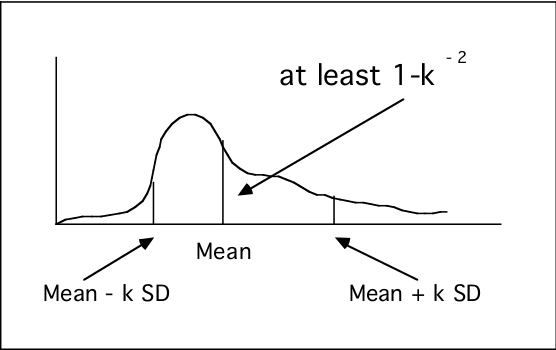
\includegraphics[width=.5\textwidth]{chapters/2_statistics/01_fundamental_probability_concepts/1_images/1_ineqChebyGraph.png}
	\end{center}
	\caption{Illustration of Chebychev inequality}
	\label{fig:fig2.01.1}
\end{figure}



\paragraph{Markov inequality}
\begin{center}
		$X\neq\underline{0}\Rightarrow \Prob{X\geq t}\leq \dfrac{\E{X}}{t}$
\end{center}
\paragraph{Theorem weak law of large numbers:}
Let $\prth{X}{i}{1}{n}\text{: independent \& identically distributed RV}$
\begin{center}
	$\lm{n}{\infty}\Prob{\left|\overline{S}_{n}-\mu\right|\geq\epsilon}=0$ with $\overline{S}_{n}=\dfrac{1}{n}\su{ {i=1}}{n}X_{i}$
\end{center}
\paragraph{Convergence in probability}
Suppose $\prth{X}{i}{1}{n}$ is a sequence of random variables de-
fined on a sample space S. The sequence ``converges in probability'' to the
random variable X if, for any $\epsilon>0$
\begin{center}
	$\lm{n}{\infty}\Prob{\left|X_{n}-X\right|<\epsilon}=1$
\end{center}
\paragraph{Convergence almost surely}
Suppose the RV $X\text{ and }\prth{X}{i}{1}{n}$ is a sequence of random variables de-
fined on a sample space S. The sequence $X_{n}(\omega)$ ``converges almost surely'' to $X(\omega)$ if
\begin{center}
	$\Prob{w\in S|\lm{n}{\infty}X_{n}(\omega)=X(\omega)}=1$
\end{center}
\paragraph{Properties}
\begin{itemize}
	\item For a Bernoulli distribution, $\overline{S}_{n}\text{ converges in probability to }p$
	\item For a Normal distribution, $\overline{S}_{n}\text{ converges almost surely to }\mu$
\end{itemize}


\subsection{Central Limit Theorem}
The central limit therorem (Lindeberg-Levy Theorem) states that for any
population distribution, the distribution of the standardized sample mean
is approximately standard normal with better approximations obtained with
the larger sample size.
\begin{center}
    $\begin{cases}\prth{X}{i}{1}{n}\hookrightarrow ?(\mu,\sigma^{2})\\ n\rightarrow\infty\end{cases} \Rightarrow \dfrac{\overline{X}-\mu}{\frac{\sigma}{\sqrt{n}}} \hookrightarrow \mathcal{N}(0, 1)$
\end{center}
\subsection{Convergence in distribution}
Consider $X$ with its cumulative density function $F$ and $\prth{X}{i}{1}{n}$ with their 
cdf $\left( F_{i} \right)_{1\leq i\leq n}$:
\begin{center}
	$\lm{n}{\infty}F_{n}(x)=F(x)\Rightarrow X_{n}\text{ "converges in distribution" to }X$
\end{center}
\subsection{Lévy Continuity Theorem}
\begin{center}
	$
	\begin{cases}	
		\prth{X}{i}{1}{n}\text{RV}\\
		\prth{F}{i}{1}{n}\text{distribution functions}\\
		\left( M_{X_{i}} \right)_{1\leq i\leq n}\text{moment generating function}
	\end{cases}$
	$\forall t\in [-h,h]\lm{n}{\infty}M_{X_{n}}(t)=M_{X}(t)\Rightarrow
	\lm{n}{\infty}F_{n}(x)=F(x)
	$
\end{center}

\section{Bivariate case}
\paragraph{Joint probability density function}
Let $\left(X,Y\right):\left(\Omega_{X},\Omega_{Y}\right)\rightarrow\left(R_{X},R_{Y}\right)$ and $f:R_{X}\times R_{Y}\rightarrow \mathbb{R}$
\begin{center}
	$\forall (x,y)\in R_{X}\times R_{Y},f(x,y)=\Prob{X=x,Y=y}\Leftrightarrow\text{ f is the joint probability density function for }X\text{ and }Y$
\end{center}

\paragraph{Marginal probability density function}
Let for all $(x,y)\in R_{X}\times R_{Y}$: $f(x,y)$ be the joint probability density of $X$ and $Y$
\begin{center}
$\begin{cases}
	f_{1}(x)=\Su{{-\infty}}{\infty}f(x,y)dy\text{is the marginal probability density of }X\\
	f_{2}(y)=\Su{{-\infty}}{\infty}f(x,y)dx\text{is the marginal probability density of }Y
\end{cases}$
\end{center}
\paragraph{Joint cumulative probability distribution function}
Let $F:\mathbb{R}^{2}\rightarrow\mathbb{R}$
\begin{center}
	$\forall (x,y)\in \mathbb{R}^{2},F(x,y)=\Prob{X\leq x,Y\leq y}=\Su{ {-\infty}}{y}\Su{ {-\infty}}{x}f(u,v)dudv\Leftrightarrow\text{ F is the joint cumulative probability density function for }X\text{ and }Y$
\end{center}
From the fundamental theorem of calculus:
$f(x,y)=\dfrac{\partial^{2}F(x,y)}{\partial x\partial y}$


\paragraph{Conditional expectation}
The conditional mean of $X$ given $Y=y$ is defined as:
\begin{center}
\fr{
$
\E{X|y}=
\begin{cases}
\su{{x\in R_{X}}}{}xg(x/y)\Leftarrow X\text{ discrete}\\
\Su{{-\infty}}{\infty}xg(x/y)dx\Leftarrow X\text{ continuous}
\end{cases}
$}
\end{center}

Properties:
\begin{center}
	$\begin{cases}
        \mathbb{E}_{X}\left(\mathbb{E}_{y|x}\left(Y|X\right)\right)=
        \mathbb{E}_{y}\left(Y\right)\\
	\E{Y|\left\{ X=x \right\}}=\mu_{Y}+\rho\dfrac{\sigma_{Y}}{\sigma_{X}}(x-\mu_{X})
	\end{cases}$	
\end{center}


\paragraph{Conditional Variance}
\begin{center}
	$\begin{cases}
	\V{Y|x}=\E{Y^{2}|x}-\E{Y|x}^{2}\\
	\mathbb{E}_{x}\left( \V{Y|X}=(1-\rho^{2})\V{Y} \right)
	\end{cases}$
\end{center}

\subsection{Distribution function}
\paragraph{Definition of probability density function (pdf):}
Let $R_{X}$ be the space of the random variable $X$. The function:
$f:R_{X}\rightarrow \mathbb{R}$ defined by:
\begin{align*}
    f(x) &= \Prob{X=x} \text{ if } X \text{ is discrete.}\\
    f(x) &= \Prob{X\in A}=\Su{A}{{}}f(x)dx \text{ if } X \text{ is continuous, with } A
    \text{ a set of real numbers.}
\end{align*}
is called probability density function of $X$.


\paragraph{Definition of cumulative density function (cdf):}
Let $R_{X}$ be the space of the random variable $X$. The function:
$F:R_{X}\rightarrow \mathbb{R}$ defined by:\\
\begin{align*}
    F(x) &= \Prob{X\leq x} \text{ if } X \text{ is discrete.}\\
    F(x) &= \Prob{X\leq x}=\Su{-\infty}{x}f(t)dt \text{ if } X \text{ is continuous, 
    with } A \text{ a set of real numbers.}
\end{align*}


\paragraph{Percentile for continuous random variables.}
Let $p\in [0;1]$, a $100p^{th}$ percentile of the distribution of a random
variable $X$ is $q\in\mathbb{R}$ satisfying:
\begin{center}
	$\Prob{X\leq q}\leq p$\\
	(Recall that the $F$ is a monotonically increasing function, then it has an 
	inverse $F^{-1}$)\\
	$q = F^{-1}(p)$
\end{center}
A $100p^{th}$ is a measure of location for the probability distribution in
the sense that $q$ divides the distribution of the probability mass into
2 parts, one having probability mass $p$ and other having probability mass
$1-p$
\begin{figure}[H]
	\begin{center}
		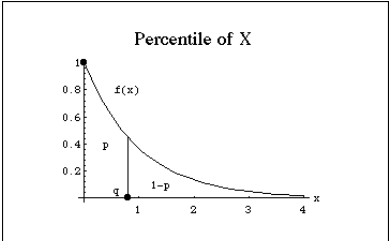
\includegraphics[width=.5\textwidth]{./chapters/2_statistics/01_fundamental_probability_concepts/2_images/1percentile.png}
	\end{center}
	\caption{Percentile}
	\label{fig:fig2.1}
\end{figure}
The $50^{th}$ percentile of any distribution is called median of the distribution.



\section{Distributions}
\subsection{Discrete distributions with finite support}
\paragraph{Bernoulli}
\paragraph{Rademacher}
\paragraph{Binomial}
\paragraph{Beta-Binomial}
\paragraph{Degenerate}
\paragraph{Uniform}
\paragraph{Hypergeometric}
\paragraph{Negative Hypergeometric}
\paragraph{Poisson Binomial}
\paragraph{Fisher's noncentral hypergeometric}
\paragraph{Benford's law}
\paragraph{Zipf's law}
\paragraph{Zipf-Mandelbrot law}







\section{Bayesian approach}
\subsection{Components}
\subsection{Bayesian concept learning}
Let be $\mathcal{D}$ the data, $h$ the hypothesis taken in account
\subsection{Likelihood}
$p\left(\mathcal{D}|h\right)$ the probability to get the observed data considering the 
hypothesis $h$.
\subsection{Prior}
$p(h)$ the probability of our hypothesis, many prior can be used, and this 
\textbf{subjective} aspect of Bayesian reasoning is a source of much controversy.

\subsection{Posterior}
The posterior is simply the likelihood times the prior, normalized.
\begin{center}
\tR{$p\left(h|\mathcal{D}\right) = \dfrac{p\left(\mathcal{D}|h\right)\times p(h)}{
    \su{h'\in\mathcal{H}}{}p\left(\mathcal{D}, h'\right)p(h')
}$}
\end{center}


\subsection{Summarizing posterior distributions}
\subsection{MAP (Maximum A Posteriori) estimation}
Although most appropriate choice for:\\
$
\begin{cases}
	\text{Real valued quantity} &\rightarrow \text{\emph{posterior median or mean}}\\
	\text{Discrete} &\rightarrow \text{\emph{vector of posterior marginals}}
\end{cases}
$\\
The most popular choice is \tB{\emph{posterior mode}} aka \tR{MAP}, because it reduces to
optimization problems for which efficient algorithms often exist.\\
Some point to be aware about MAP:
\begin{itemize}
	\item \uB{No measure of uncertainty}
	\item \tB{Plugging in the MAP estimate can result in overfitting}
	\item \tB{The mode is an untypical point}, unlike the mean or median the mode is a
		point of measure 0, it does not take the volume of the space into account.
	\item \tB{MAP estimation is not invariant to reparameterization}, for example 
		passing from centimeters to inches can break things.)\\ The MLE does not
		suffer from this since the likelihood is a function not a probability
		density
\end{itemize}


\subsection{Credible intervals}
With point estimates, we want a measure of confidence. 
\tB{
$$ C_{\alpha}\left(\mathcal{D}\right) = (l, u): \Prob{{l\leq \theta \leq u | \mathcal{D}}} \geq 1 - \alpha
$$}
In general, credible intervals are usually what people want to compute but confidence
intervals are usually what they actually compute, because most people are taught 
frequentist statistics but not Bayesian statistics.\\
Sometimes with central intervals there might be points be outside the CI which have higher
probability density.\\
More formally $p^{*}$ such that: 
\begin{center}
	$1-\alpha = 
	\Su{{\theta:p(\theta|\mathcal{D})>p^{*}}}{}p(\theta|\mathcal{D})d\theta$
\end{center}
Then the \uB{HPD} such that:
\begin{center}
	$\mathcal{D}=\left\{\theta: p(\theta|\mathcal{D})\geq p^{*}\right\}$
\end{center}


\subsection{Bayesian Model Selection}
A more efficient approach than cross-validation, meaning fitting \emph{k} times each
model, is \tR{to compute the posterior over models}.
$$
p(m|\mathcal{D}) = \dfrac{p(\mathcal{D}|m)p(m)}{\su{{m\in\mathcal{M}}}{}p(m|\mathcal{D})}
$$
From this we can compute the \tB{MAP model $\hat{m} = \displaystyle \argmax_{m}
p(m|\mathcal{D})$}\\
Then we have the \tB{marginal likelihood}: $p(\mathcal{D}|\hat{m}) = \Su{}{}p(
\mathcal{D}|\hat{m})p(\theta|\hat{m})d\theta$

\paragraph{Baysian Occam's razor}
\tB{In integrating out the parameters rather than maximizing them we are automatically 
protected from overfitting}: model with more parameters do not necessarily have higher 
marginal likelihood.\\
A way to understand the Bayesian Occam's razor effect is to \tB{remember that 
probabilities must sum to one, meaning $\su{{\mathcal{D}'}}{}p(\mathcal{D}'|m)=1$. Complex
models, which can predict many things, must spread their probability mass thinly, and 
hence will not obtain as large a probability for any given data set as simpler models.}

\paragraph{Computing the marginal likelihood (evidence)}
For a fixed model we often write:
$$p(\bm{\theta}|\mathcal{D},m) \propto p(\bm{\theta}|m)p(\mathcal{D}|\bm{\theta},m)$$
This valid since $p(\mathcal{D}|m)$ is constant. However when comparing models we need
to know how to compute the marginal likelihood, $p(\mathcal{D}|m)$. In general this can
be quite hard, since we have to integrate over all possible parameter values, but when
we have a conjugate prior, it is easy to compute.\\
Let $p(\bm{\theta})=\dfrac{q(\bm{\theta})}{Z_{0}}$ be our prior, where $q(\bm{\theta})$
is an unnormalized distribution, and $Z_{0}$ is the normalization constant of the prior.
Let $p(\mathcal{D}|\bm{\theta})=\dfrac{q(\mathcal{D}|\bm{\theta})}{Z_{l}}$ be the 
likelihood, where $Z_{l}$ contains any constant factors in the likelihood. Finally let
$p(\bm{\theta}|\mathcal{D})=\dfrac{q(\bm{\theta}|\mathcal{D})}{Z_{N}}$ be our posterior
where $q(\bm{\theta}|\mathcal{D})=q(\mathcal{D}|\bm{\theta})q(\bm{\theta})$ is the 
unnormalized posterior, and $Z_{N}$ is the normalization constant of the posterior.\\
We have:
$
\begin{cases}
	p(\bm{\theta})= \dfrac{p(\mathcal{D}|\bm{\theta})p(\bm{\theta})}{p(\mathcal{D})}\\
	\dfrac{q(\bm{\theta}|\mathcal{D})}{Z_{N}} = \dfrac{q(\mathcal{D}|\bm{\theta})
	q(\bm{\theta})}{Z_{l}Z_{0}p(\mathcal{D})}\\
	p(\mathcal{D}) = \dfrac{Z_{N}}{Z_{0}Z_{l}}
\end{cases}
$

 
Simpler approach
\begin{itemize}
	\item \textbf{BIC} In general $p(\mathcal{D}|m) = \Su{}{}p(\mathcal{D}|\bm{\theta})p(\bm{\theta}|m)d\bm{
\theta}$ can be quite difficult to compute. A popular approximation is:
		\tB{$BIC \triangleq \log(p(\mathcal{D}|\bm{\hat{\theta}_{MLE}})) - 
		\dfrac{dof(\bm{\hat{\theta}_{MLE}})}{2}\log(N)\approx\log{p(\mathcal{D})}$}
	\item \textbf{AIC}:
		\tB{$AIC(m,\mathcal{D})\triangleq\log(p(\mathcal{D}|\bm{\hat{\theta}}_{MLE
		})) -dof(m)$}\\
		This is derived from Frequentist framework and cannot be interpreted as 
		an approximation to the marginal likelihood. The penalty of AIC is less
		than BIC, it causes AIC pick more complex models. That \tB{can be better for 
		predictive accuracy}.
	\item Effect of the prior.\\
		If the prior is unknown, the correct Bayesian procedure is to put a prior
		on the prior. That is we should put a prior on the hyper-parameter 
		$\alpha$ as well as the parameters $\bm{w}$. To compute the marginal 
		likelihood we should integrate out all unknowns, we should compute:
		\tB{$\Su{}{}\Su{}{}p(\mathcal{D}|\bm{w})p(\bm{w}|\alpha,m)p(\alpha|m)
		d\bm{w}d\alpha$}
		A computational shortcut is to optimize $\alpha$ rather than integrating
		it out. That is, we use \tG{$p(\mathcal{D}|m)\approx\Su{}{}p(\mathcal{D}
		\bm{w})p(\bm{w}|\alpha,m)d\bm{w}$}.
		where \tG{$\hat{\alpha} = \displaystyle \argmax_{\alpha} p(\mathcal{D}|
			\alpha,m) = \displaystyle \argmax_{\alpha}\Su{}{}p(\mathcal{D}|
		\bm{w})p(\bm{w}|\hat{\alpha},m)d\bm{w}$}
\end{itemize}
\paragraph{Bayes Factors}
When prior on models is uniform, then model selection is equivalent to picking the model
with the highest marginal likelihood. Now suppose we just have two models we are 
considering, call them the null hypothesis, $M_{0}$ and the alternative hypothesis,
$M_{1}$.\\
\tB{$$BF_{1,0} \triangleq \dfrac{p(\mathcal{D}|M_{1})}{p(\mathcal{D}|M_{0})}=
    \dfrac{\left.\frac{p(M_{1}|\mathcal{D})}{p(M_{0}|\mathcal{D})}\right\}\text{\emph{Posterior odds}}}{\left.\frac{p(M_{1})}{p(M_{0})}\right\}\text{\emph{Prior odds}}}
$$}
\begin{itemize}
    \item \emph{Posterior odds}: quantifies relative plausibility of the rival hypotheses
        \textbf{after} having seen the data.
    \item \emph{Bayes Factor}, $BF_{1,0}$, quantifies the evidence provided by the data, 
        this is like a likelihood ratio, except we integrate out the parameters, which 
        allows us to compare models of different complexity.
    \item \emph{Prior odds}: quantifies relative plausibility of the rival hypotheses
        \textbf{before} seeing the data.
\end{itemize}

 

\begin{table}[h!]
	\begin{tabular}{|cl|}
		\hline
	\textbf{Bayes Factor} $\bm{BF(1,0)}$ & \textbf{Interpretation}\\
		\hline
		$BF<\frac{1}{100}$ & Decisive evidence for $M_{0}$\\
		\hline
		$BF<\frac{1}{10}$ & Strong evidence for $M_{0}$\\
		\hline
		$\frac{1}{10}<BF<\frac{1}{3}$ & Modest evidence for $M_{0}$\\
		\hline
		$\frac{1}{3}<BF<1$ & Weak evidence for $M_{0}$\\
		\hline
		$1<BF<3$ & Weak evidence for $M_{1}$\\
		\hline
		$3<BF<10$ & Modest evidence for $M_{1}$\\
		\hline
		$BF>10 $ &  Strong evidence for $M_{1}$\\
		\hline
		$BF>100$ & Decisive evidence for $M_{1}$\\
		\hline
	\end{tabular}
\end{table}


\paragraph{Jeffreys-Lindley paradox}
Problems can arise when we use improper priors (i.e. priors that do not integrate to 1)
for model selection/ hypothesis testing, even though such priors may be acceptable for 
other purposes. \tB{In particular the Bayes Factor will always favor the simplest model 
since the probability of the observed data under a complex model with a very diffuse prior
will be very small.} Thus it is important to use proper priors when doing model selection.

 
\subsection{Priors}
The most controversial aspect of Bayesian statistics is its reliance on priors
\subsection{Uninformative priors}
If we do not have strong evidence on what $\theta$ should be, it is common to use an
uninformative priors, to "let the data speak for itself".\\
One might think that the most uninformative prior would be the uniform distribution: 
$Beta(1, 1)$, but the posterior would then be: $\E{\theta|\mathcal{D}} =
\dfrac{N_{1}+1}{N_{1}+N_{0}+2}$, whereas the MLE is $\dfrac{N_{1}}{N_{1}+N_{0}}$.\\
As by decreasing the magnitude of the pseudo counts, we can lessen the impact of the 
prior, we can argue that the most non-informative prior is: 
$$\lm{\epsilon}{0} Beta(\epsilon, \epsilon) = Beta(0, 0)$$
Called the \emph{Haldane prior}, it is an improper prior.\\
In general it is advisable to perform a some kind of sensitivity analysis, in which one
checks how much one's conclusions or prediction change in response to change in the 
modelling assumptions which includes the choice of the prior and the likelihood as well.
If the conclusion are relatively insensitive to the modelling assumption, one can have
more confidence in the results.
\subsection{Jeffreys priors}
Harold Jeffreys designed a general purpose technique for creating non-informative priors.
The key observation is that if $p(\phi)$ is non-informative then any re-parametrization
of the prior, such as $\theta=h(\phi)$ for some function $h$ should also be 
non-informative.
\begin{itemize}
	\item Start with a variable change: $p_{\theta}(\theta) = p_{\phi}(\phi)\left|\dfrac{d\phi}{d\theta}\right|$
	\item Consider the following constraint: $p_{\phi}(\phi)\propto
		\sqrt{\mathcal{I}(\phi)}$, where $\mathcal{I}(\phi)$ is the Fisher 
		information.\\ $\mathcal{I}(\phi) \triangleq - \E{2 \times 
		\dfrac{d\log\left(p(X|\phi)\right)}{d\phi}}$. This a measure of the
		curvature of the expected negative log likelihood and hence a measure of
		stability of the MLE.
	\item Now $\dfrac{d\log(p(x|\theta))}{d\theta} = 
		\dfrac{d\log(p(X|\phi))}{d\phi}\dfrac{d\phi}{d\theta}$
	\item $\mathcal{I}(\theta) = \mathcal{I}(\phi)
		\left(\dfrac{d\phi}{d\theta}\right)^{2}$
	\item $\sqrt{\mathcal{I}(\theta)} = \sqrt{\mathcal{I}(\phi)}\left|\dfrac{d\phi}
		{d\theta}\right|$
	\item Finally $p_{\theta}(\theta) = p_{\phi}(\phi)\left|\dfrac{d\phi}
		{d\theta}\right| \propto \sqrt{\mathcal{I}(\phi)}\left|\dfrac{d\phi}
		{d\theta}\right| = \sqrt{\mathcal{I}(\theta)}$
\end{itemize}

\subsection{Robust priors}
To prevent an undue influence on the result, we build priors having heavy tails, which 
avoids forcing things to be too close to the prior mean.

\subsection{Mixture of conjugate priors}
Conjugate priors simplify the computation of robust priors, but are often not robust, and 
not flexible enough to encode our prior knowledge. However it turns out that a mixture of
conjugate priors is also conjugate, and seem to be a good compromise.



\subsection{Hierarchical and Empirical Bayes}
\paragraph{Hierarchical Bayes}
A key requirement for computing the posterior $p(\theta|\mathcal{D})$ is the 
specification of a prior $p(\theta|\eta)$ where $\eta$ are the hyper-parameters. A 
Bayesian approach is to \tB{put a prior on our priors}. This is an example of a \textbf{
hierarchical Bayesian Model}.

\paragraph{Empirical Bayes}
In hierarchical Bayesian models, we need to compute the posterior on multiple levels of
latent variables. For example, in a two-level model, we need to compute:
$p(\eta, \theta|\mathcal{D}) \propto p(\mathcal{D}|\theta)p(\theta|\eta)p(\eta)$\\
\tB{We can approximate the posterior on the hyper-parameters with a point-estimate, 
$p(\eta|\mathcal{D})\approx \delta_{\hat{\eta}}(\eta)$ where $\hat{\eta}=\argmax_{\eta}
p(\eta|\mathcal{D})$. Since $\eta$ is typically much smaller than $\theta$ in 
dimensionality, it is less prone to overfitting, so we can safely use a uniform prior on 
$\eta$}. Then the estimate becomes: 
$$ \hat{\eta} = \argmax_{\eta} p(\mathcal{D}|\eta) = \argmax_{\eta} \Su{}{}
p(\mathcal{D}|\theta)p(\theta|\mathcal{\eta})d\theta $$
This overall approach is called \textbf{Empirical Bayes}\\
Empirical Bayes violates the principle that the prior should be chosen independently of 
the data. However, we can just view it as a computationally cheap approximation to 
inference in a hierarchical Bayesian model, just as we viewed MAP estimation as an approximation to inference in the one level model $\theta \rightarrow \mathcal{D}$. In fact, we
can construct a hierarchy in which the more integrals one performs, the "more Bayesian" 
one becomes:
\begin{center}
	\begin{tabular}{|*{2}{l|}}
		\hline
		\textbf{Method} & \textbf{Definition} \\
		\hline
		Maximum likelihood & $\hat{\theta} = \argmax_{\theta} 
		p(\mathcal{D}|\theta)$ \\
		\hline
		MAP estimation & $\hat{\theta} = \argmax_{\theta} 
		p(\mathcal{D}|\theta)p(\theta|\eta)$ \\
		ML-II (Empirical Bayes) & $\hat{\eta}=\argmax_{\eta}\Su{}{}
		p(\mathcal{D}|\theta)p(\theta|\eta)d\theta = \argmax_{\eta}p(\mathcal{D}|
		\eta)$ \\
		\hline
		MAP-II & $\hat{\eta}=\argmax_{\eta}\Su{}{}
		p(\mathcal{D}|\theta)p(\theta|\eta)p(\eta)d\theta = \argmax_{\eta}p(
		\mathcal{D}| \eta)p(\eta)$\\
		\hline
		Full Bayes & $p(\theta, \eta|\mathcal{D}) \approx p(\mathcal{D}|\theta)
		p(\theta|\eta)p(\eta)$\\
		\hline
	\end{tabular}
\end{center}



\subsection{Bayesian Decision Theory}
\tB{We can formalize any given statistical decision problem as a game against nature} (as 
opposed to a game against other strategic players, which is the topic of game theory).
\tB{In this game, nature picks a state or parameter or label, $y\in \mathcal{Y}$, unknown
to us, and then generates an observation, $\bm{x}\in\mathcal{X}$ which we get to see. We
then have to make a decision, that is, we have to choose an action $a$ from some 
\textbf{action space} $\mathcal{A}$. Finally we incur some \textbf{loss}, $L(y, a)$, which
measures how compatible our action $a$ is with nature's hidden state $y$.}\\
Our goal is to devise a decision procedure or policy, $\delta: \mathcal{X}\rightarrow
\mathcal{A}$ which specifies the optimal action for each possible input which specifies the optimal action for each possible input, meaning the action that minimizes the expected 
loss:
$$ \delta(\bm{x}) = \argmin_{{a\in \mathcal{A}}} \E{{L(y, a)}}$$
In the Bayesian vision, the expected value of $y$ given the data we have seen so far, 
whereas in the frequentist vision the expected value refers to $x$ and $y$ that we expect
to see in the future.\\
\tO{In the Bayesian vision the optimal action having observed $\bm{x}$ is defined as the 
action $a$ that minimizes the \textbf{posterior expected loss}:
$$ \rho(a|\bm{x})\triangleq\mathbb{E}_{p(y|x)}\left(L(y, a)\right) = \su{y}{}L(y, a)
p(y|x)$$}
Hence the \tR{Bayes estimator also called Bayes decision rule is given by:
$$\delta(\bm{x}) = \argmax_{a\in\mathcal{A}}\rho(\bm{a}|\bm{x})$$}

\subsection{Bayes estimators for common loss functions}
\begin{itemize}
    \item \textbf{MAP} estimate minimizes 0-1 loss: $L(y, a) = \mathbb{I}_{y\neq a}
		\begin{cases}
			0 \text{ if } a = y\\
			1 \text{ else}
		\end{cases}$
    \item \textbf{Reject option}, in classification problems where $p(y|\bm{x})$ is very 
		uncertain we may prefer to choose a reject action, in which we refuse to 
		classify the example as any of the specified classes. Let choosing $a=C+1$
		correspond to picking the reject action, and choosing $a\in\{1,...,C\}$
		correspond to picking one of the classes.\\
		$L(y=j, a=i) = 
		\begin{cases}
			0 &\text{ if } i=j \text{ and } i,j\in\{1,...,C\}\\
			\lambda_{r} &\text{ if } i=C+1 \\
			\lambda_{s} &\text{ otherwise}
		\end{cases} $\\
		where $\lambda_{r}$ is the cost of the reject action, and $\lambda_{s}$ is
		the cost of a substitution error. 
    \item \textbf{Squared Error ($l_{2}$)} for a continuous parameters. $L(y, a) =
        (y-a)^{2}$
    \item \textbf{Absolute Error ($l_{1}$)} more robust against outliers. $L(y,a)=
		\lvert y-a\rvert$. The optimal point is the median.
    \item \textbf{Supervised learning} considering a prediction function $\delta: 
        \mathcal{X} \rightarrow \mathcal{Y}$ and some cost function $l(y, \delta(x))$. 
        Then the loss incurred by taking action $\delta$ when the unknown state of nature
        is $\theta$ (the parameters of the data generating the mechanism).
        $L(\bm{\theta}, \delta) \triangleq 
        \mathbb{E}_{(\bm{x}, y)~p(\bm{x},y|\bm{\theta})}\left(
        l(y, \delta(\bm{x}))\right)=\su{\bm{x}}{}\su{y}{}L\left(y,\delta(\bm{x}) 
        p(\bm{x},y|\bm{\theta})\right)$
\end{itemize}

\subsection{Model evaluation metrics}
\begin{itemize}
    \item \textbf{False positive vs False negative trade-off} for binary decision problems
        three are 2 types of errors:
        \begin{enumerate}
            \item {false positive} (false alarm) if $\hat{y}=1 \wedge y=0$
            \item {false negative} (missed detection) if $\hat{y}=0 \wedge y=1$
        \end{enumerate}
        We can consider the loss matrix:\\
        \begin{tabular}{|*{3}{c|}}
            \hline
            \textbf{Headers} & $\bm{y=1}$ & $\bm{y=0}$\\
            \hline
            $\bm{\hat{y}=1}$ & 0 & $L_{FP}$\\
            \hline
            $\bm{\hat{y}=0}$ & $L_{FN}$ & 0\\
            \hline
        \end{tabular}
        where $L_{FN}$ is the cost of a false negative and $L_{FP}$ the cost of a false
        positive.

    \item \textbf{ROC curves} From the below table \\
        \begin{tabular}{|cc|*{3}{c|}}
            \hline
            \multicolumn{2}{|c}{\textbf{Headers}} & \multicolumn{2}{|c|}{\textbf{Truth}} &
            \textbf{Count}\\
            \hline
            \multirow{2}{*}{\textbf{Estimate}} & 1 & $TP$ & $FP$ & $\hat{N}_{+}=TP + FP$\\
                                               & 0 & $FN$ & $TN$ & $\hat{N}_{-}=FN + TN$\\
            \hline
            \multicolumn{2}{|c|}{\textbf{Count}} & $N_{+}=TP+FN$ & $N_{-}=FP+TN$ 
                                               & $N=N_{+}+N_{-}=\hat{N}_{+}+\hat{N}_{-}$\\
            \hline
        \end{tabular}\\
        we can generate the \emph{confusion matrix} is the below table\\
        \begin{tabular}{|*{3}{c|}}
            \hline
            \textbf{Headers} & $\bm{y=1}$ & $\bm{y=0}$\\
            \hline
            $\bm{\hat{y}=1}$ & $\dfrac{TP}{N}$ (sensitivity/recall) 
                           & $\dfrac{FP}{N}$ (error type I/ false alarm) \\
            \hline
            $\bm{\hat{y}=0}$ & $\dfrac{FN}{N}$ (error type II/ missed detection) 
                           & $\dfrac{TN}{N}$ (specificity) \\
            \hline
        \end{tabular}
    \item \textbf{Precision recall curves}
        When trying to detect a rare event the number of negatives is very large, hence
        comparing \emph{sensitivity} and \emph{the error of type I} is not very 
        informative. We would then like to use a measure that only talks about positives.
        \begin{itemize}
            \item \textbf{precision} $=\dfrac{TP}{\hat{N}_{+}}$
            \item \textbf{recall} $=\dfrac{TP}{N_{+}}$
        \end{itemize}
        A \textbf{precision recall curve} is a plot of \textit{precision} vs 
        \textit{recall}.
    \item \textbf{F-scores} is the \emph{harmonic mean of precision and recall}:\\
        $F_{1} \triangleq \dfrac{2}{\frac{1}{precision} + \frac{1}{recall}}$
\end{itemize}





\section{Frequentist approach}
\subsection{Sampling distribution}
\paragraph{Sampling Distributions of an estimator}
\tB{In frequentist statistic a parameter estimate $\hat{\theta}$ is computed by applying 
an estimator $\delta$ to some data $\mathcal{D}$}, so \textbf{$\hat{\theta}=\delta(
\mathcal{D})$}.
The \tR{uncertainty in the parameter estimate can be measured by computing the 
\emph{sampling distribution of the estimator}}.
Imagine sampling many different \tB{datasets $\mathcal{D}^{(s)}$ from some true model 
$p(\cdot|\theta^{*})$ meaning $\mathcal{D}^{(s)}=\left\{x_{i}^{(s)}\hookrightarrow 
p(\cdot|\theta^{*})\right\}_{1\leq i\leq N}$ for $1\leq s\leq S$ and $\theta^{*}$ is the 
true parameter. Now apply the estimator $\hat{\theta}(\cdot)$ to each $\mathcal{D}^{(s)}$
to get a set of estimates $\{\hat{\theta}(\mathcal{D}^{(s)})\}_{1\leq s\leq S}$.}\\
\tR{As we late $S \rightarrow \infty$, the distribution induced on $\hat{\theta}(\cdot)$ 
is the \textbf{sampling distribution of the estimator}.}

\paragraph{Bootstrap}
It is a \tB{simple \emph{Monte Carlo} technique to approximate the sampling distribution}.
The idea is that \tR{if we knew the true parameters $\theta^{*}$, we could generate $S$ 
fake datasets of size $N$}, from the true distribution. We could then \tR{compute our 
estimator from each sample, and use the empirical distribution of the resulting samples as
our estimate of the sampling distribution}.\\
Since $\theta$ is unknown, the idea of the \tB{\textbf{parametric bootstrap} is to 
generate the samples using $\hat{\theta}(\mathcal{D})$ instead}.
An alternative, called \tB{\textbf{non-parametric bootstrap} is to sample the $x_{i}^{s}$
(with replacement) from the original data $\mathcal{D}$ and then compute the induced
distribution} as before.


\subsection{Fequentist decision theory}
In Frequentist decision theory there is a loss function and a likelihood, but there
is no prior and hence no posterior or posterior expected loss. Thus there is no 
automatic way of deriving an optimal estimator, unlike the Bayesian case.\\
\uB{Instead, we are free to choose any estimator or decision procedure $\delta: 
\mathcal{X} \rightarrow \mathcal{A}$ we want}.\\
Having chosen an estimator, we define its \tR{expected loss or risk} as follows
\tR{
\begin{center}
 $R(\theta^{*}, \delta) \triangleq \mathbb{E}_{p(\tilde{\mathcal{D}}|\theta^{*})}
\left(L(\theta^{*}, \delta(\tilde{\mathcal{D}}))\right) = \Su{}{}L\left(\theta^{*},
\delta(\tilde{\mathcal{D}})\right)p(\tilde{\mathcal{D}})d\tilde{\mathcal{D}}$   
\end{center}
}
where $\tilde{\mathcal{D}}$ is data sampled from 'nature's distribution' represented by
parameter $\theta^{*}$.\\
Whereas the \tR{Bayesian posterior expected loss}: 
\tR{
\begin{center}
    $p(a|\mathcal{D, \pi}) \triangleq \mathbb{E}_{p(\theta|\mathcal{D},\pi)}\left(
        L(\theta, a)\right) = \Su{\Theta}{}L(\theta, \bm{a})p(\theta|\mathcal{D}, \pi)
        d\theta
    $
\end{center}
}
We see that the Bayesian approach averages over $\theta$, which is unknown, and conditions
on $\mathcal{D}$ which is known. Unlike the frequentist approach averages over $\tilde{
\mathcal{D}}$, thus ignoring the observed data, and conditions on $\theta^{*}$ which is 
unknown.

\subsection{Bayes risk}
How to chose amongst the estimators? 
We need some way to convert $R(\theta^{*}, \delta)$ into single measure of quality, $R(
\delta)$ which does not depend on knowing $\theta^{*}$. One approach is to \uR{put a prior
on $\theta^{*}$ and then to define} \tR{\textbf{Bayes risk}} of an estimator as follows:
\tR{
\begin{center}
    $R_{B}(\delta) \triangleq \mathbb{E}_{p(\theta^{*})}\left(R(\theta^{*}, \delta)\right)
    =\Su{}{}R(\theta^{*}, \delta)p(\theta^{*})d\theta^{*}$
\end{center}
}
A \tR{\textbf{Bayes estimator} or \textbf{Bayes decision rule}} is one which minimizes the
expected risk: \tR{$\delta_{B} \triangleq \displaystyle\argmin_{\delta} R_{B}(\delta)$}

\subparagraph{Connection Bayesian and Frequentist approaches to decision theory.}
\begin{itemize}
    \item \emph{Theorem 1} \uB{A Bayes estimator can be obtained by minimizing the 
            posterior expected loss for each $\bm{x}$}
    \item \emph{Theorem 2} \tB{Every admissible frequentist decision rule is a Bayes 
            decision rule with respect to some possibly improper prior distribution}.
\end{itemize}

\subparagraph{Minimax risk}
Some frequentist statistic users avoid using Bayes risk since it requires the choice of
a prior, although this is only in the evaluation of the estimator, not necessarily as 
part of its construction. An alternative approach is as follows:
\begin{enumerate}
    \item Define the  maximum risk of an estimator as:\\
        $R_{max}(\delta) \triangleq \displaystyle\max_{\theta^{*}}R(\bm{\theta}^{*},
        \delta)$
    \item A \tB{\textbf{minimax rule}} is one which minimizes the maximum risk:
        \tB{$\delta_{MM} \triangleq \displaystyle\argmin_{\delta} R_{\max}(\delta)$} 
\end{enumerate}
\uB{Minimax estimators have a certain appeal, however computing them can be hard and 
furthermore they are very pessimistic}.
In most statistical situations, excluding games theoretic ones, assuming nature is an
adversary is not a reasonable assumption.


\subsection{Admissible estimators}
The basic problem with frequentis decision theory is that it relies on knowing the true
distribution $p(\cdot|\theta^{*})$ in order to evaluate the risk. However it might be 
the case that some estimators are worse than others regardless of the value of 
$\theta^{*}$.\\
In particular \tB{if for $\theta \in \Theta, R(\theta, \delta_{1}) \leq R(\theta, 
    \delta_{2})$ then we say that $\delta_{1}$ \textbf{dominates} $\delta_{2}$}.\\
An estimator is said to be \textbf{admissible} if it is not strictly dominated by any 
other estimator.\\
\textbf{Admissibility is not enough}


\subsection{Desirable properties of estimators}
\subsection{Consistent estimators}
An estimator is said to be \textbf{consistent} \tB{if it eventually recovers the true
parameters that generated the data as the sample size goes to infinity}. 

\subsection{Unbiased estimator}
The \textbf{bias} of an estimator is defined as 
\tR{
\begin{center}
    $bias\left(\hat{\theta}(\cdot)\right) = \mathbb{E}_{p(\mathcal{D}|\theta^{*})}
    \left(\hat{\theta}(\mathcal{D})-\theta^{*}\right)$
\end{center}
}
The estimator is \tB{unbiased when the bias is equal to 0}.

\subsection{Minimum variance estimators}
A famous result called the \textbf{Cramerè-Rao lower bound} provides a lower bound on the
variance of any unbiased estimator. More precisely:
Let $\left(X_{j}\right)_{1 \leq j \leq p} \hookrightarrow p(X|\theta_{0})$ and 
\tB{$\hat{\theta}(\cdot)$ an unbiased estimator of $\theta^{*}$}
Then, under various smoothness assumptions on $p(X|\theta_{0})$ we have  
\tR{
\begin{center}
    $\mathbb{V}(\hat{\theta}) \geq \dfrac{1}{nI(\theta^{*})}$
\end{center}
}
where \tB{$I(\theta^{*})$ is the Fisher information matrix}.

\subsection{Bias-Variance Trade-off} 
As $MSE = variance + bias^{2}$\\
\tB{It might be wise to use a biased estimator, so long as it reduces our variance},
assuming our goal is to minimize squared error. 


\subsection{Empirical Risk Minimization}
\subsection{Frequentist issue}
\tB{Frequentist decision theory suffers from the fundamental problem that one cannot 
actually compute the risk function, since it relies on knowing the true data 
distribution}. By contrast, the Bayesian posterior expected loss can always be computed 
since it conditions on the data rather that on $\theta^{*}$.\\
\uB{However there is one setting which avoids this problem, it is when the task is to 
predict observable quantities, as opposed to estimating hidden variables or parameters}.\\
\tB{Instead of looking at loss functions of the form $L(\bm{\theta^{*}}, 
\delta(\mathcal{D}))$ let us look at loss functions of the form $L(y, \delta(\bm{x}))$}.\\
Then the risk becomes:
$R(p_{*}, \delta) \triangleq \mathbb{E}_{(\bm{x}, y)\hookrightarrow p_{*}}\left(L(y,
\delta(\bm{x}))\right) = \su{\bm{x}}{}\su{\bm{y}}{}L(y, \delta(\bm{x}))p_{*}(\bm{x}, y)$
Where $p_{*}$ represents "nature's distribution", indeed this distribution is unknown, 
but a simple approach is to use the empirical distribution, derived from some training 
data to approximate $p_{*}(x,y)\approx
p_{emp}(x,y) \triangleq \dfrac{1}{N}\su{i=1}{N}\delta_{x_{i}}(\bm{x})\delta_{y_{i}}(y)$
We define the empirical risk as follows:
\tR{
\begin{center}
    $R_{emp}(\mathcal{D}, \mathcal{D}) \triangleq R(p_{emp}, \delta) = \dfrac{1}{N}
    \su{i=1}{N}L(y_{i}, \delta(\bm{x}_{i}))$
\end{center}
}


\subsection{Regularized risk minimization}
\begin{center}
    $R'(\mathcal{D}, \delta) = R_{emp}(\mathcal{D}, \delta) + \lambda C(\delta)$
\end{center}
where $C(\delta)$ measures the complexity of the prediction function $\delta(\bm{x})$ and 
$\lambda$ controls the strength of the complexity penalty. 
This approach is known as \textbf{regularized risk minimization}.


\subsection{Components}
\subsection{Introduction}
Avoid treating parameters as randome variables.
The notion of variation across repeated trials forms the basis for modelling
uncertainity.


\subsection{Hypothesis Testing}
A \emph{frequentist} statistics, probabilities represent the frequencies at which 
particular events happen.

\subsection{\emph{p-value}}
It is the heart of frequentist hypothesis testing, it tells us the \tB{probability of 
getting a particular test statistic $t$ as big as the one we have or bigger under the null
hypothesis} (that there is actually no effect).\\
By convention we usually conclude an effect is \emph{statistically significant} if the 
\emph{p-value} is less than a threshold $\alpha$.

\subsection{Confidence intervals}
When we fit a model to our data we look for the \emph{maximum of likelihood} parameters,
meaning the parameters that are most consistent with our data. 
For each parameter we will able to construct $95\%$ interval namely \tB{$95$ of the $100$ 
intervals generated will contain the true value of the parameter}.\\
If $H_{0}: \beta=0$ is true, the probability of getting a $95\%$ confidence interval that
does not include 0 is less than 0.05. In other words, if the $95\%$ confidence does not 
include 0, $p<0.05$.
\begin{figure}[H]
	\begin{center}
		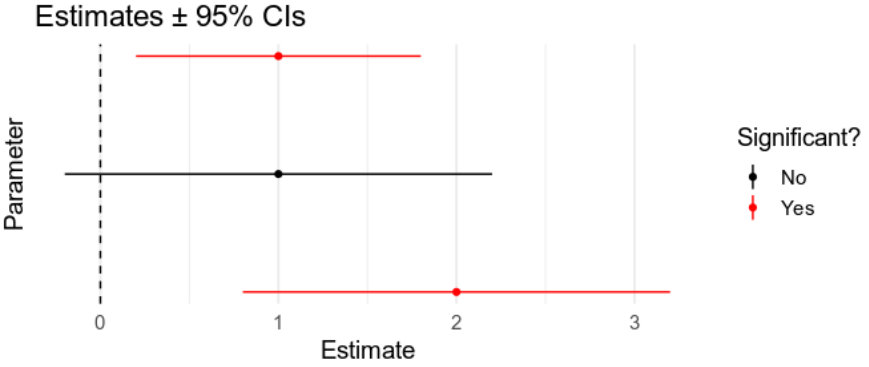
\includegraphics[width=\textwidth]{./chapters/2_statistics/04_frequentist_approach/4_images/1_estimates.png}
	\end{center}
	\caption{Confidence interval}
	\label{fig:2.4.1_estimates}
\end{figure}

\subsection{Multiple comparisons}
The more tests we run the more likely it is to we'll find at least one that is significant
even though the null hypothesis is true. We can then apply a Bonferroni correction.\\
Let's say we are running $k$ tests, we can either adjust: 
\begin{itemize}
	\item the threshold $\alpha_{adj} = \dfrac{\alpha}{k}$ OR
	\item the \emph{p-value} $p_{ajd} = k\times p$
\end{itemize}






\section{Common statistical tests}
\subsection{Use of statistical tests}
\subsection{Terms}
\begin{itemize}
    \item \emph{Paired} samples: one-to-one correspondence between data in the first and
        second set.
    \item \emph{Matched} samples: every subject in one group with an equivalent in 
        another.
\end{itemize}


\subsection{Table of statistical hypothesis test}
\label{statistical_method_table}{Statistical method table.}\\ 
\begin{tabular}{|*{4}{b{4cm}|}}
\hline
& \textbf{Binomial/Discrete} & \textbf{Continuous, from Normal distribution} & 
\textbf{Continuous measurement\newline (Score/Rank), from non-Normal distribution} \\
\hline
    \textbf{Example of data sample} & List of patients recovering or not after a 
    treatment & Reading of heart pressure from several patients & Ranking of several
    treatment efficiency\\
\hline
    \textbf{Describe one data sample} & Proportions & Mean, Standard Deviation & Median \\
    \hline
    \emph{Compare one data sample to a hypothetical distribution} & $\chi^{2}$ / \emph{G-test} or \label{binomial_test}{Binomial test} & 1-sample t-test & Sign test or Wilconox test \\
    \hline
    \emph{Compare 2 paired samples} & Sign test & Paired t-test & Sign test or Wilconox test \\
    \hline
    \emph{Compare 2 unpaired samples} & $\chi^{2}$ / \emph{G-test} or Fisher's extract test & Unpaired t-test & Mann-Whitney test \\
    \hline
    \emph{Compare 3 or more unmatched samples} & $\chi^{2}$ / \emph{G-test} & 1-way ANOVA & Kruksal-Wallis test \\
    \hline
    \emph{Compare 3 or more matched samples} & Cochrane Q test & Repeated-measures ANOVA & Friedman test\\
    \hline
    \emph{Quantify association between 2 paired samples} & Contingency coefficients & Pearson correlation & Sperman correlation \\
    \hline
\end{tabular}


\subsection{List of common statistical test}
\subsection{\hyperref[binomial_test]{Binomial}}
To check if the deviations from a theoretically expected distribution of observations into
2 categories.\\

\paragraph{Assumptions}
\begin{itemize}
    \item \tB{Sample items are independent.}
    \item Items are dichotomous and nominal.
    \item The sample size is significantly less than the population size
    \item The sample is a fiar representation of the population
\end{itemize}


\paragraph{Frequentist}
Let define a user-defined probability $p_{0}$, with $H_{0}: p = p_{0}$ and
$\begin{cases}
    H_{1}: p \neq p_{0}\text{: two-tailed test} \\
    H_{1}: p < p_{0}\text{: left-tailed test} \\
    H_{1}: p > p_{0}\text{: right-tailed test} \\
     
\end{cases}$

\paragraph{Bayesian}
Define the prior distribution with a \emph{Beta}($a,b$) distribution\\

\textit{\hyperref[statistical_method_table]{Return to the table.}}


\subsection{$\chi^{2}$ test}
Either used to test \emph{goodness-of-fit} and \emph{independence} between 2 variables.
It checks either if there is a significant difference between the expected and observed 
frequencies.
\begin{itemize}
    \item \emph{goodness-of-fit}: expected frequencies are computed with a theoretical 
        relationship between observed frequencies
    \item \emph{independence}: expected frequencies are computed with observed frequencies
        from the other sample
\end{itemize}
\paragraph{Assumptions}
\begin{itemize}
    \item simple random sample
    \item sample with a sufficiently large size is assumed, for small sample size see Cash test
    \item expected cell count has to be adequate, a rule of thumb is at least 5 for 2-by-2
        table and 5 or more in 80\% of cells in larger tables.
    \item Independence of the observations
\end{itemize}

\paragraph{Frequentist}
$\chi^{2} = \su{i=1}{n}\dfrac{\left(\frac{O_{i}}{N} - p_{i} \right)^{2}}{p_{i}}
\begin{cases}
    O_{i}\text{: number of observations of type }i \\
    N\text{: total number of observations}\\
    n\text{: number of cells in the table.}
    p_{i}\text{: expected proportions of the fraction of type}i\text{ in the population.}
\end{cases}
$

\paragraph{Bayesian}
Does not exist, see \emph{contingency table}\\

\textit{\hyperref[statistical_method_table]{Return to the table.}}


\subsection{Exact test of goodness-of-fit}
Unlike the conventional statistical tests, there is no \emph{test statistic}, we directly
compute the \emph{p-value} under the null hypothesis.
The most common use are for dichotomous nominal variables or multinomial variables.

\paragraph{Assumptions}
\begin{itemize}
    \item \tB{Observations are independent.}
    \item Small sample size $\lessapprox 1000$
\end{itemize}

\paragraph{Frequentist}
Let us define the list of, respectively, expected counts for each modality 
$i,~(E_{i})_{1\leq i\leq m}$, and observed counts $(O_{i})_{1\leq i\leq m}$.
Then
$\begin{cases}
    \bm{H_{0}: \forall i\in \inter{1}{m},~O_{i} = E_{i}}\\
    H_{1}: \exists i\in \inter{1}{m},~O_{i} \neq E_{i}\text{: two-tailed test} \\
\end{cases}$




\subsection{Fisher's exact test}
To check the significance of the contingency between 2 kinds of classification of a given
object, \uB{initially Fisher used this test to distinguish drink in which the tea has been
put before the milk or vice-versa}. For large sample use \emph{G-test}

\paragraph{Assumptions}
\begin{itemize}
    \item In practice, small sample size $\lessapprox 1000$
\end{itemize}

\paragraph{Frequentist}
For example let's divide a population into male and female and for each persons indicating
if this person is currently studying or not. We want to test if the proportion of studying
students is higher among the women than among the men.
\begin{center}
    \begin{tabular}{|*{4}{c|}}
    \hline
    & \textbf{Men} & \textbf{Women} & \textbf{Row Total}\\
    \hline
    \textbf{Studying} & $a$ & $b$ & $a+b$ \\
    \hline
    \textbf{Non-Studying} & $c$ & $d$ & $c+d$ \\
    \hline
    \textbf{Column Total} & $a+c$ & $b+d$ & $a + b + c + d = n$ \\
    \hline
    \end{tabular}
\end{center}
The conditional on the margins of the table is distributed as $\text{\emph{Hypergeometric}}(a+c, a+b, c+d)$ meaning $a + c$ draws from a population with $a + b$ success and $c+d$ 
failures.
The probability of obtaining such set of values is given by
\begin{center}
    $p = \dfrac{{{a+b}\choose{a}}\times{{c+d}\choose{c}}}{{{n}\choose{a+c}}}
    = \dfrac{{{a+b}\choose{b}}\times{{c+d}\choose{d}}}{{{n}\choose{b+d}}}$
\end{center}

\paragraph{Bayesian}
Does not exist, see \emph{contingency table} \\

\textit{\hyperref[statistical_method_table]{Return to the table.}}


\subsection{G-test}

It's a likelihood-ratio or a maximum likelihood statistical significance test. 
Either used to test \emph{goodness-of-fit} and \emph{independence} between 2 variables.
It checks either if there is a significant difference between the expected and observed 
frequencies. This test tends to replace $\chi^{2}$\emph{-test}
\begin{itemize}
    \item \emph{goodness-of-fit}: expected frequencies are computed with a theoretical 
        relationship between observed frequencies
    \item \emph{independence}: expected frequencies are computed with observed frequencies
        from the other sample
    \item \emph{repeated tests}: first variable is analysed with a goodness-of-fit and the
        second one represents the repetition of the experiments multiple times. Thus it
        allows to assess the goodness-of-fit on a large sample instead of multiple lower
        samples. Expected frequencies is a theoretical relationship between the observed
        frequencies segmented in groups by the modalities of the second variable.
\end{itemize}


\paragraph{Assumptions}
\begin{itemize}
    \item 
    \item Expected count must not be small in any modality.
\end{itemize}

\paragraph{Strengths}
\begin{itemize}
    \item Approximation to the theoretical $chi^{2}$ distribution is better attained with
        \emph{G-test} than $\chi^{2}$ \emph{test}.
    \item Cases where $O_{i} > 2\times E_{i}$, \emph{G-test} is always better than
        $\chi^{2}$ \emph{test}.
\end{itemize}

\paragraph{Weaknesses}
\begin{itemize}
    \item in test of independence, for a small sample size use rather Fisher's extract 
        test.
\end{itemize}


\paragraph{Frequentist}
We compare the observed counts in each modality with their expected counts.
Let us define the list of, respectively, expected counts for each modality 
$i,~(E_{i})_{1\leq i\leq m}$, and observed counts $(O_{i})_{1\leq i\leq m}$.
Then
$\begin{cases}
    \bm{H_{0}: \forall i\in \inter{1}{m},~O_{i} = E_{i}}\\
    H_{1}: \exists i\in \inter{1}{m},~O_{i} \neq E_{i}\text{: two-tailed test} \\
\end{cases}$

\begin{center}
    $G = 2\su{i=1}{m}O_{i}\times\ln\left(\dfrac{O_{i}}{E_{i}}\right)$
\end{center}

$$
\ln\left(\dfrac{L(\tilde{\theta}|x)}{L(\hat{\theta}|x)}\right)
= \ln\left(\dfrac{\prd{i=1}{m}\tilde{\theta}^{x_{i}}}{\prd{i=1}{m}\hat{\theta}^{x_{i}}}\right)
= \ln\left(\dfrac{\prd{i=1}{m}\left(\frac{x_{i}}{n}\right)^{x_{i}}}{\prd{i=1}{m}\left(\frac{e_{i}}{n}\right)^{x_{i}}}\right)
= \ln\left(\prd{i=1}{m}\left(\dfrac{x_{i}}{e_{i}}\right)^{x_{i}}\right)
= \su{i=1}{m}x_{i}\ln\left(\dfrac{x_{i}}{e_{i}}\right)
$$

Then we multiply by $-2$ to get \emph{G-test} that is asymptotically equivalent to the 
\emph{Pearson's} $\chi^{2}$ formula.


\subsection{Cochran's Q test}
It checks if $k$ treatments have identical effect, the response can take only 2 possible 
outcomes and a second variable segments the treatments.

\begin{center}
    \begin{tabularx}{.65\textwidth}{|*{5}{c|}}
    \hline
     & \textbf{Treatment 1} & \textbf{Treatment 2} & $\cdots$  & \textbf{Treatment k}\\
    \hline
    \emph{Block 1} & $x_{11}$ & $x_{12}$ & $\cdots$  & $x_{1k}$\\
    \hline
    \emph{Block 2} & $x_{21}$ & $x_{22}$ & $\cdots$  & $x_{2k}$\\
    \hline
    \emph{Block 3} & $x_{31}$ & $x_{32}$ & $\cdots$  & $x_{3k}$\\
    \hline
    $\vdots$ & $\vdots$ & $\vdots$ & $\ddots$ & $\vdots$ \\
    \hline
    \emph{Block b} & $x_{b1}$ & $x_{b2}$ & $\cdots$  & $x_{bk}$\\
    \hline
    \end{tabularx}
\end{center}
And $\forall (i,j)\in\inter{1}{b}\times\inter{1}{k}, x_{ij}\in\left\{0, 1\right\}$

\paragraph{Assumptions}
\begin{itemize}
    \item The blocks are randomly selected from the population of all possible blocks.
    \item Outcome of the treatments are dichotomous, and should be coded in a standard way
\end{itemize}

\paragraph{Frequentist}
For example if $b$ respondents in a survey had each been asked $k$ \emph{Yes/No} questions
the \emph{Q-test} could be use to test the null hypothesis that all questions were equally
likely to elicit the answer "Yes".\\
We have
$\begin{cases}
    H_{0}\text{: the treatments are equally effective} \\
    H_{a}\text{: the treatments are \emph{not} equally effective} 
\end{cases}$

\begin{center}
    $
    T = k(k-1)\dfrac{\su{j=1}{k}\left(x_{\cdot j} - \frac{N}{k}\right)^{2}}{
    \su{i=1}{b}x_{i\cdot}\left(k-x_{i\cdot}\right)}
    \begin{cases}
        k\text{: number of treatments} \\
        x_{\cdot j}\text{: column total for the }j\text{th treatment} \\
        b\text{: number of blocks} \\
        X_{i\cdot}\text{: row total for the }i\text{th block} \\
        N\text{: grand total}
         
    \end{cases}$
\end{center}

For significance level $\alpha$, the asymptotic critical region is 
$T > \chi^{2}_{1-\alpha, k-1}$ which is the ($a-\alpha$) quantile of the $\chi^{2}$ 
distribution with $K-1$ degrees of freedom.

\paragraph{Bayesian}
Does not exist, see \emph{contingency table} \\



\subsection{Sign test}
It is a statistical method to test for consistent differences between pairs of 
observations, such as the weight of subjects before and after treatment.
For comparisons of paired observations $(x, y)$ the \emph{sign-test} is most useful if 
comparison can only be expressed as $x>y,~x=y,\text{ or } x<y$.
If instead the differences can be expressed in numeric quantities it is worthy to use 
\emph{t-test} or \emph{Wilcoxon signed-rank test} will usually have greater power than
the sign test to detect consistent differences.

\paragraph{Frequentist}
Let $p=\Prob{X>Y}$, then
$\begin{cases}
    H_{0}:~p=0.5\text{ meaning that given a random pair of measurements }(x_{i}, y_{i})
    \text{ then }x_{i}\text{ and }y_{i}\text{are equally likely to be larger than the
    other}\\
    H_{a}:~p\neq 0.5
\end{cases}$
Pairs are omitted for which there is no differences so that there is a potential reduced
sample of $m$ pairs.\\
The statistics $W$ is defined as follow:
\begin{center}
    $W = \mathbf{1}_{\left\{x_{i} > y_{i}\right\}} \hookrightarrow \mathcal{B}(m, 0.5)$
\end{center}

\paragraph{Assumptions}
Let $\forall i\in\inter{1}{n},~Z_{i} = X_{i} - Y_{i}$

\begin{itemize}
    \item $Z_{i}$ are assumed independent.
    \item Each $Z_{i}$ comes from the same continuous population.
    \item The values $X_{i}$ and $Y_{i}$ are ordered.
\end{itemize}

\paragraph{Strengths}
\begin{itemize}
    \item A fewer assumptions need to be made than for parametrical test
\end{itemize}

\paragraph{Weaknesses}
\begin{itemize}
    \item The power of test is lower than for a parametrical test
\end{itemize}



\subsection{Contingency coefficients: Cramér's V}
To quantify associations between 2 paired samples in a contingency table, it is based
on $\chi^{2}$ and varies from 0 (no association) to 1 (complete association).
\paragraph{Frequentist}
Let a sample of size $n$ of the simultaneously distributed variable $A$ and $B$.
$\forall (i,j)\in\inter{1}{r}\times\inter{1}{c},~n_{ij} = \text{\emph{Card}}\left(
\left\{A_{i},B_{j}\right\}\right)$.
Then $\chi^{2} = \su{(i,j)\in\inter{1}{r}\times\inter{1}{c}}{}\dfrac{\left(n_{ij} - \frac{
n_{i\cdot}\times n_{\cdot j}}{n}\right)^{2}}{\frac{n_{i\cdot}\times n_{\cdot j}}{n}}$\\
Finally the Cramér's V with bias correction is: 
\begin{center}
    $V = \sqrt{\dfrac{\max\left(0, \frac{\chi^{2}}{n} - \frac{(r-1)(c-1)}{n}\right)}{\min\left(r-\frac{(r-1)^{2}}{n-1}-1, c-\frac{(c-1)^{2}}{n-1}-1\right)}}$
\end{center}

\paragraph{Assumptions}
\begin{itemize}
    \item The both variables have to be nominal.
\end{itemize}

\paragraph{Strengths}
\begin{itemize}
    \item Good analog of the $R^{2}$ for categorical variables.
\end{itemize}

\paragraph{Weaknesses}
\begin{itemize}
    \item Can tend to overestimate the strength of association.
\end{itemize}



\subsection{Contingency table from a Bayesian perspective}
To test the independence hypothesis between 2 variables.
\paragraph{Bayesian}
Let's consider 4 sampling plans, depending on which sampling plan is chosen the Bayes
factor formula will change.
\begin{itemize}
    \item \emph{Poisson} sampling scheme: Each cell count is considered as random and so
        is the grand total, the cells are Poisson distributed. This design often occurs
        in purely observational work.
    \item \emph{Joint multinomial} sampling scheme: same as above except that now, the 
        grand total is fixed. 
    \item \emph{Independent multinomial} sampling scheme: either all row margins or all 
        column margins are fixed, this scheme is frequently used in psychological studies.
    \item \emph{Hypergeometric} sampling scheme: here both row margins and column margins are fixed. Practical use of this scheme is rare!  
\end{itemize}
Bayes factors are often difficult to compute, as they are obtained by integrating out over
the entire parameter space, a process that is non-trivial when the integrals are 
high-dimensional and intractable. \\
Then we will use the 4 Bayes Factor developed by \emph{Gunnel and Dickey in 1974}, because
they only require computation of common functions such as gamma functions, for which 
numerical approximation are already available.\\
Here the logic: the Bayes Factor $BF^{i+1}_{01}$ computed at the observation $i+1$, 
contains the information up to the step $i$ with the extra information of the step $i+1$. 
We can then see $BF^{i+1}_{01}$ as the Bayes factor of the observation $i+1$ conditioned
on the observation $i$.\\
Finally thanks to the successive conditionalization the Bayes Factor are easy to compute.

\paragraph{Assumptions}
\begin{itemize}
    \item We need to be consider data providing from one of the following sampling scheme: \emph{Poisson}, \emph{Joint multinomial}, \emph{Independent multinomial} or 
        \emph{Hypergeometric}
\end{itemize}

\paragraph{Strengths}
\begin{itemize}
    \item Bayesian approach, then no issue to assess the significance
    \item Implemented in R
\end{itemize}

\paragraph{Weaknesses}
\begin{itemize}
    \item Restricted to the above sampling scheme today. 
\end{itemize}


\subsection{Wilconox test}
Non parametric test, used to test the location of a population based on a data sample or 
to compare the locations of two populations using two matching samples.\\
It is a good alternative of the \emph{t-test} when the mean is not of interest for the 
studied population.
\paragraph{Frequentist}
Let $Y$ and $X$ be 2 random variables, and $\left(x_{i}, y_{i}\right)_{1\leq i\leq n}$
a paired sample. 
\begin{enumerate}
    \item $\forall i\in\inter{1}{n},~\left|x_{i}\right|$
    \item Sort the $\left(\left|x_{i}\right|\right)_{1\leq i\leq n}$ and assign a rank
        $\left(R_{i}\right)_{1\leq i\leq n}$
    \item The test statistic i $T=\su{i=1}{n}sgn\left(X_{i}\right)R_{i}$
    \item Produce a \emph{p-value} by computing T to its distribution under the null
        hypothesis.
\end{enumerate}
We will provide the logic for a one-sample test, the two-sample follows the same logic but
with 2 variables.

Assume the data consists of independent and identically distributed (IID) samples from a
distribution $F$ then consider 2 variables $(X_{1}, X_{2})\hookrightarrow IID(F)$
Define $p_{2} = \Prob{\dfrac{X_{1} + X_{2}}{2}>0} = 1-F^{(2)}(0)$
Then Wilcoxon signed-rank \emph{sum} $\rightarrow H_{0}:~p_{2} = \dfrac{1}{2}$
In restricting the distributions of interest we can reach more interpretable null and 
alternative hypotheses. On mildly restrictive is that $F^(2)$ has a unique median $\mu$. 
This median is called pseudo median of $F$
Then we have $H_{0}:~\mu=0$
\begin{itemize}
    \item  
\end{itemize}


\paragraph{Assumptions}
\begin{itemize}
    \item Distribution $F$ is symmetric
\end{itemize}

\paragraph{Strengths}
\paragraph{Weaknesses}

TO COMPLETE

\subsection{Mann-Whitney test}
Test for a randomly selected values $x$ and $y$ from 2 populations, $\Prob{x\leq y} = 
\Prob{x > y}$
\paragraph{Frequentist}
Let $(n_{1}, n_{2})\mathcal{N}_{*}^{2}$ and $\left(x_{i}\right)_{1\leq i\leq n_{1}}$
and $\left(y_{i}\right)_{1\leq i\leq n_{2}}$ both samples independent of each other.\\
Then
$\begin{cases}
    U_{1} = n_{1}n_{2} + \frac{n_{1}(n_{1} + 1)}{2} - R_{1} \\
    U_{2} = n_{1}n_{2} + \frac{n_{2}(n_{2} + 2)}{2} - R_{2} 
\end{cases}$
$R_{1}, R_{2}$ being the sum of the ranks in groups 1 and 2. \\
Note that $AUC_{1}=\dfrac{U_{1}}{n_{1}n_{2}}$ meaning \emph{U}-statistics is related to
the area under the receiver operating characteristic.


\paragraph{Assumptions}
\begin{itemize}
    \item All observation from both groups are independent
    \item Values are at least ordinal
    \item $H_{0}$: the distribution of both population is identical
    \item $H_{1}$: the 2 distribution of population are different
\end{itemize}

\paragraph{Strengths}
\paragraph{Weaknesses}

\subsection{Kruksal-Wallis test}
Non-parametrical to test if samples originate from the same distribution.
\paragraph{Frequentist}
Let $N$ be the number of observations across all groups, $g$ number of groups, $n_{i}$ the
number of observation in the group $i$, $r_{ij}$ the rank of observation $j$ from group 
$i$.\\
And 
$\begin{cases}
    \overline{r}_{i\cdot} = \dfrac{\su{j=1}{n_{i}}r_{ij}}{n_{i}} \\
    \overline{r} = \dfrac{N + 1}{2}
\end{cases}$
\begin{itemize}
    \item Rank all data from all groups together
    \item $\left(N-1\right)\dfrac{\su{i=1}{g}n_{i}\left(\overline{r}_{i\cdot} - 
                \overline{r}\right)^{2}}{\su{i=1}{g}\su{j=1}{n_{j}}n_{i}\left(r_{ij} - 
        \overline{r}\right)^{2}}$
        To actually check the stochastic differences.
    \item A correction can be brought for large number of ties.

\end{itemize}

\paragraph{Assumptions}
\begin{itemize}
    \item Independence
    \item All groups should have te same distributions
\end{itemize}

\paragraph{Strengths}
\begin{itemize}
    \item Non-parametrical test, no need of the normally distributed assumption.
\end{itemize}

\paragraph{Weaknesses}

\subsection{Friedman test}
Non-parametric statistical test, analogu of the \emph{repeated-measures ANOVA}.
It use to detect differences in treatments across multiple test attempts.
\paragraph{Frequentist}
\begin{itemize}
    \item Consider a matrix of $n$ rows (the blocks) and $k$ columns (the treatments)
    and a single observation at the intersetion of each block and treatment. Then 
    calculate the ranks.
    \item $\overline{r}_{\cdot j} = \dfrac{1}{n}\su{i=1}{n}r_{ij}$
    \item The test statistic is given by $Q = \dfrac{12n}{k(k+1)}\su{j=1}{k}\left(\overline{r}_{\cdot j} - \dfrac{k+1}{2}\right)^{2}$
    Note that the value of $Q$ does need to be adjusted for tied values in data.
    \item Finally when n or k is large ($n>15 or k>4$) the probability distribution of $Q$ can be approximated by
    a $\chi^{2}$ distribution.
\end{itemize}

\paragraph{Assumptions}
\begin{itemize}
    \item Independence
\end{itemize}
\paragraph{Strengths}
\paragraph{Weaknesses}

\subsection{Sperman test}
It assesses how well the relationship between 2 variables can be described using a monotonic function.
Let $X, Y$ be 2 random variables, and $R$ the function transforming the realization of a random variable.

\paragraph{Frequentist}
$r_{s} = \rho_{R(X), R(Y)} = \dfrac{Cov\left(R(X), R(Y)\right)}{\sigma_{R(X)}\sigma_{R(Y)}}
\begin{cases}
\rho:\text{ Pearson correlation coefficient applied to the rank variables} \\
Cov\left(R(X), R(Y)\right)
\end{cases}$
\paragraph{Assumptions}
\paragraph{Strengths}
\paragraph{Weaknesses}

\subsection{Pearson correlation coefficient}
This coefficient is essentially a normalized measurement of the covariance such that the result
has a value $-1$ and 1
\paragraph{Frequentist}
$\rho_{X, Y} = \dfrac{Cov\left(X, Y\right)}{\sigma_{X}\sigma_{Y}}$
\paragraph{Assumptions}
\paragraph{Strengths}
\paragraph{Weaknesses}
\begin{itemize}
    \item Not robust
\end{itemize}

\subsection{Repeated-measures ANOVA}
Used in repeated measure design, meaning when we measure multiple time the same variable
taken on the same or matched subject either under different conditions or at different periods.
\paragraph{Frequentist}
Here $F = \dfrac{\frac{SS_{treatment}}{df_{treatment}}}{\frac{SS_{error}}{df_{error}}}$
In a \emph{between-subjects} design there is a element of variance due to individual difference that 
is combined with the treatment and error term, meaning: $SS_{total} = SS_{treatment} + SS_{error}$
In a \emph{repeated-measure} design it is possible to partition subject variability from the
treatment and error term, meaning $SS_{total} = SS_{treatment(excluding indivdual differences) + SS_{subjects} + SS_{error}}$

\paragraph{Assumptions}
\begin{itemize}
    \item \emph{Normality}: for each level of the within-subject factor, the dependent variable must have a normal distribution.
    \item \emph{Sphericity}: difference scores computed between 2 levels of a within subject factor must have the same variance
    for the comparison of any 2 levels.
    \item \emph{Randomness}: cases should be derived from a random sample.
\end{itemize}
\paragraph{Strengths}
\begin{itemize}
    \item ability to partition out variability due to individual differences.
\end{itemize}
\paragraph{Weaknesses}
\begin{itemize}
    \item Vulnerable to missing values, imputation, unequivalent time points
    between subjects and violation of Sphericity.
\end{itemize}

\subsection{1-way ANOVA}
Analysis of Variance describes \uB{the partition of the response variable sum of squares in a 
linear model into ``explained'' and ``unexplained'' components.}\\
\begin{itemize}
	\item Single categorical (or less common numerical) explanatory variable corresponds to One-Way ANOVA
	\item 2 factors to Two-Way ANOVA
	\item 3 factors to Three-Way ANOVA
\end{itemize}
The term ``analysis of variance'' is a bit of misnomer, \tB{we use variance-like quantities to
study the equality or non-equality of population means}, so we are analyzing means, not variances.
\paragraph{Frequentist}
\tR{examines equality of population means for a quantitative outcome and a 
single categorical explanatory variable with any number of levels}.\\
The term \tB{``one-way'' indicates that there is a single explanatory variable (``treatment'') 
with 2 or more levels and only one level of treatment is applied at any time for a given subject}.\\
And $H_{0}:\forall (i,j) \in \inter{1}{k}^{2} \mu_{i} = \mu_{j}$


In ANOVA \uB{we work with variances and also ``variance-like quantities'' which are not really the
variance of anything}, but are still calculated as $\frac{SS}{df}$ all of these quantities are
called ``mean squares''.\\

The deviation for subject $j$ of group $i$ in the figure above is mathematically equal to $Y_{ij}-
\overline{Y}_{i}$ where $Y_{ij}$ is the observed value for subject $j$ of group $i$ and $\overline{Y}_{i}$ is the sample mean for group $i$.
\begin{figure}[H]
	\begin{center}
		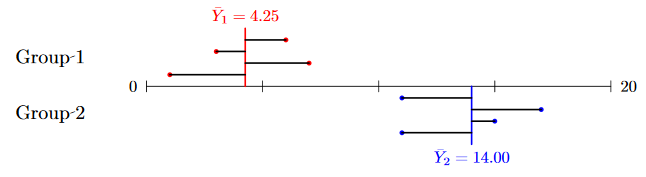
\includegraphics[width=\textwidth]{./chapters/2_statistics/05_common_statistical_tests/2_images/1_anova_inter_grp.PNG}
	\end{center}
	\caption{Deviations for within-group of squares}
	\label{fig:3_anovaInterGrp}
\end{figure}
\begin{center}
\fr{
$ MS_{within} = \dfrac{SS_{within}}{df_{within}}
\begin{cases}
	SS_{within} = \su{{j=1}}{k}SS_{j}=\su{{j=1}}{k}\su{{i=1}}{n_{j}}\left(Y_{ij}-\overline{Y}_{\bullet j}
	\right)\\
	df_{within} = df_{j} = \su{{j=1}}{k}(n_{j}-1) = N-k
\end{cases}
$
}\end{center}

\tB{$MS_{within}$ is a good estimate of $\sigma^{2}$ from our model regardless of the truth of 
$H_{0}$.} This is due to the way $SS_{within}$ is defined.

\begin{figure}[H]
	\begin{center}
		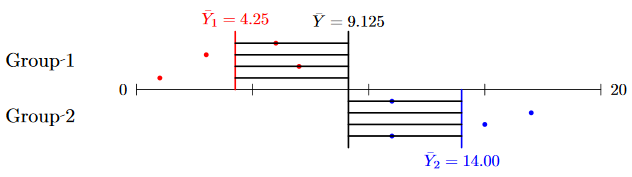
\includegraphics[width=\textwidth]{./chapters/2_statistics/05_common_statistical_tests/2_images/2_anova_btw.PNG}
	\end{center}
	\caption{Deviations for betwwen-group sum of squares}
	\label{fig:4_anovaBtw}
\end{figure}
$SS_{between}$ is the sum of the $N$ squared between-group deviations, where the deviation is
the same for all subjects in the same group. The formula is : 
\begin{center}
\fr{
$
MS_{Between} = \dfrac{SS_{Between}}{df_{between}}
\begin{cases}
SS_{between} = \su{{j=1}}{k}n_{j}\left(\overline{Y}_{\bullet j}-\overline{Y}\right)^{2}\\
df_{between} = k-1
\end{cases}
$
}\end{center}
Because of the way $SS_{between}$ is defined, \tB{$MS_{between}$ is a good estimate of $\sigma^{2}
$ only if $H_{0}$ is true}. Otherwise it tends to be larger. \\
The $F-statistic$ defined by $F=\dfrac{MS_{between}}{MS_{within}}$ \uR{tends to be larger if the
alternative hypothesis is true than if the null hypothesis is true}.\\

We can quantify ``large'' for the \emph{F-statistic}, by comparing it to its null sampling 
distribution which is the specific \emph{F-distribution}  which has degrees of freedom matching
the numerator and denominator of the \emph{F-statistic}.\\
Concerning inferences to build the confidence interval we need the \tB{\emph{standard error} (the
standard deviation of the means) that is $\sqrt{\dfrac{MS_{within}}{n_{i}}}$}\\

Numerically we have:\\
Given 2 samples with means $\mu_{1}$ and $\mu_{2}$, same variance $\sigma^{2}$ and $n=n_{1}+n_{2}$
observations.
Model: 
\begin{center}
	$\forall (j,i)\in\inter{1}{2}\times\inter{1}{n_{j}}y_{ij} = \mu_{i} + \epsilon_{ij} = \mu + \alpha_{j} + \epsilon_{ij}$
\end{center}
$\alpha_{j}=\mu_{j}-\mu$ is called (treatment-) effect

Decomposition:
\begin{align*}
	SS_{total} =& \su{{j=1}}{n_{1}}\left(y_{1j}-\overline{y}\right)^{2} +
	\su{{j=1}}{n_{2}}\left(y_{2j}-\overline{y}\right)^{2}\\
	=& \su{{j=1}}{n_{1}}\left(y_{1j}-\overline{y_{1}}+\overline{y_{1}}-\overline{y}\right)^{2}
	+ \su{{j=1}}{n_{2}}\left(y_{2j}-\overline{y_{2}}+\overline{y_{2}}-\overline{y}\right)^{2}\\
	=& \underbrace{(n_{1}-1)s_{1}^{2} + (n_{2}-1)s_{2}^{2}}_{SS_{within}} +
	\underbrace{n_{1}(\overline{y}_{1}-\overline{y}) + 
	n_{2}(\overline{y}_{2})-\overline{y}^{2}}_{SS_{between}}
\end{align*}
$SS_{between}$ corresponds to squared enumerator $(\overline{y}_{1} - \overline{y}_{2})^{2}$ of
the statistic: 
\begin{align*}
	SS_{between} =& n_{1}(\overline{y}_{1}-\overline{y})^{2} + 
	n_{2}(\overline{y}_{2}-\overline{y})^{2}\\
	=& n_{1}\left(\overline{y}_{1}-\dfrac{n_{1}\overline{y}_{1}+n_{2}\overline{y}_{2}}{n_{1}+
	n_{2}}\right)^{2} + n_{2}\left(\overline{y}_{2}-\dfrac{n_{1}\overline{y}_{1}+n_{2}
	\overline{y}_{2}}{n_{1}+ n_{2}}\right)^{2}\\
	=& \dfrac{n_{1}n_{2}}{n_{1}+n_{2}}\left(\overline{y}_{1}-\overline{y}_{2}\right)^{2}
\end{align*}
$SS_{within}$ corresponds to denominator of \emph{t-statistic}:
$s=\sqrt{\dfrac{(n_{1}-1)s_{1}^{2}+(n_{2}-1)s_{2}^{2}}{n_{1}+n_{2}-2}}$\\
Pooled variance that is an estimate of the fixed common variance $\sigma^{2}$ underlying various
populations that have different means.
$\hat{\sigma}=\dfrac{(n_{1}-1)s_{1}^{2}+(n_{2}-1)s_{2}^{2}}{(n_{1}-1)+(n_{2}-1)}$
Null hypothesis $H_{0}:\mu_{1}=\mu_{2}$ or $\alpha_{1}=\alpha_{2}=0$
\emph{F-test}
$\left(\overline{Y}_{1}-\overline{Y}_{2}\right)\hookrightarrow \mathcal{N}\left(\mu_{1}-\mu_{2},
\left(\frac{1}{n_{1}}+\frac{1}{n_{2}}\right)\sigma^{2}\right)\\
\E{\left[\overline{Y}_{1}-\overline{Y}_{2}\right]^{2}}=\left(\frac{1}{n_{1}}+\frac{1}{n_{2}}
\right)\sigma^{2}+(\mu_{1}-\mu_{2})^{2}\\
\E{MS_{between}}=\E{\frac{n_{1}n_{2}}{n_{1}+n_{2}}\left[\overline{Y}_{1}-\overline{Y}_{2}
\right]^{2}} = \sigma^{2}+\frac{n_{1}n_{2}}{n_{1}+n_{2}}(\mu_{1}-\mu_{2})^{2}\\
\E{MS_{whithin}}=\sigma^{2}\\
F = \dfrac{MS_{between}}{MS_{within}}$
Here $F=t^{2}$\\
\begin{align*}
	\text{Degrees of freedom} =& n - 1\\
	=& \underbrace{(n-m)}_{df_{within}} + \underbrace{(m-1)}_{df_{between}}
\end{align*}
\begin{itemize}
	\item $SS_{within}$ and $SS_{between}$ are independent
	\item under $H_{0}$ $\E{MS_{between}} = \E{MS_{within}} = \sigma^{2}$
	\item under $H_{a}$ $\E{MS_{between}}>\sigma^{2}$ and $\E{MS_{within}} = \sigma^{2}$
\end{itemize}
Hence $$ F= \dfrac{MS_{between}}{MS_{within}}\hookrightarrow F_{m-1,n-m}$$
In the case of 2 groups (``\emph{t-test}'') we received:
$$ \overline{y}_{1}-\overline{y}_{2} \pm t_{n-2,1-\frac{\alpha}{2}}s\sqrt{\frac{1}{n_{1}}+
\frac{1}{n_{2}}}$$


\paragraph{Assumptions}
\begin{center}
	The statistical model for which one-way ANOVA is appropriate is that the
	\begin{itemize}
		\item (Quantitative) Outcomes for each group are normally distributed
		\item Outcome variances are all equal to  ($\sigma^{2}$)
		\item The errors are assumed to be independent.
	\end{itemize}
\end{center}
\paragraph{Strengths}
\paragraph{Weaknesses}

\subsection{T-test}
It is commonly used when the test statistic would follow a normal distribution
if the value of a scaling term in the test statistic were known.\\
When the scaling term is estimated from the data, under certain conditions, the
test statistic follows a \emph{Student's t-test}.\\
Most test statistics have the form $t=\dfrac{Z}{s}$, $Z$ may be sensitive to 
the alternative hypothesis, whereas $s$ isa scaling parameter allowing to determine
the distribution \emph{t}.
\subsection{One-sample}
\paragraph{Frequentist}
$$
t = \dfrac{\overline{x} - \mu_{0}}{\frac{s}{\sqrt{n}}},
\begin{cases}
    \overline{x}\text{: sample mean}\\
    s\text{: sample standard deviation}\\
    n\text{: sample size}
\end{cases}
$$
By the central limit theorem, if the observations are independent and the second
moment exist, then $t$ will approximately follow the distribution $\mathcal{N}(0, 1)$

\paragraph{Assumptions}
Although the parent population does not need to be normally distributed, the distribution
of the population sample means $\left(\overline{x}_{s}\right)_{1\leq s\leq S}$.\\
\paragraph{Strengths}
\paragraph{Weaknesses}


\subsection{Slope of a regression line}
Suppose one is fitting: $Y = \alpha + \beta x + \epsilon$, where $x$ is known and $\alpha$ and $\beta$ are unknown
and finally $\epsilon \hookrightarrow \mathcal{N(0, 1)}$.
Symbols with hat will refer to estimators.
\paragraph{Frequentist}
$$t_{score} = \dfrac{\hat{\beta} - \beta_{0}}{SE_{\hat{\beta}}} \hookrightarrow \mathcal{N}(0, 1)$$

\paragraph{Assumptions}
\paragraph{Strengths}
\paragraph{Weaknesses}

\subsection{Paired / Unpaired  t-test}
Depending on if the samples are paired or not and the differences between means and variances, the formula will be different. 
It is not worthful to dive in these formulas.
\paragraph{Frequentist}
\paragraph{Assumptions}
\paragraph{Strengths}
\paragraph{Weaknesses}

Weimprove




\part{Classical Learning}
\begin{figure}[H]
    \begin{center}
        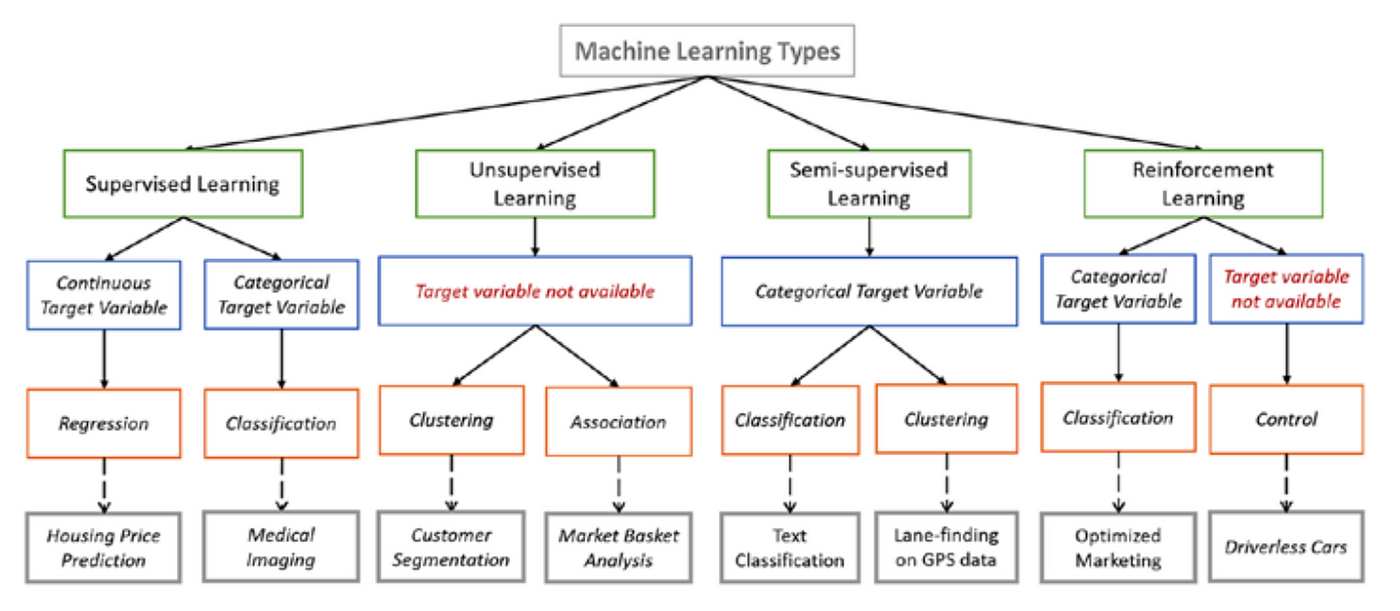
\includegraphics[width=\textwidth]{chapters/3_images/type_of_ml_methods.png}
    \end{center}
    \caption{Types of machine learning methods}
    \label{fig:type_of_ml_methods}
\end{figure}
\chapter{Supervised Learning}
With the \tB{\emph{generative} approach we create a joint model of the form $\prob{y,\bm{x}}$, and
then to condition on $\bm{x}$, thereby deriving $\prob{y|\bm{x}}$}.\\
Alternatively, \tB{fitting directly a model of the form $\prob{y|\bm{x}}$ is a \emph{
discriminative} approach}.

\begin{itemize}
    \item \emph{Easy to fit}: generative classifiers is usually very easy
    \item \emph{Fit classes separately?}: in a generative classifier we estimate the parameters 
        of each class conditional density independently
    \item \emph{Handle missing features easily?}: in a generative classifier there is a natural way
        to handle missing data: $\prob{\bm{x}_{i},r_{i}|\bm{\theta},\bm{\phi}} = \prob{r_{i}|\bm{
        x}_{i},\bm{\phi}}\prob{\bm{x}_{i}|\bm{\theta}}$ where $\bm{\phi}$ are the parameters
        controlling whether the item is observed or not. Missing completely at random (MCAR): $\prob{
        r_{i}|\bm{x}_{i},\bm{\phi}} = \prob{r_{i}|\bm{x}^{0}_{i}|\bm{\phi}}$, missing at random 
        (MAR): $\prob{r_{i}|\bm{x}_{i},\bm{\phi}} = \prob{r_{i}|\bm{x}^{0}_{i},\bm{\phi}}$
    \item \emph{Can handle unlabeled training data?}: Fairly easy in using generative models
    \item \emph{Symmetric in inputs and outputs?}: We can run a generative model "backward" and 
        infer probable inputs given the output by computing $\prob{\bm{x}|y}$
    \item \emph{Can handle feature preprocessing?}: discriminative methods allow to preprocess the
        input in arbitrary ways, by replacing $\bm{x}$ with $\phi(\bm{x})$
    \item \emph{Well-calibrated probabilities?}: discriminative models are usually better calibrated
        in terms of their probability estimates.
\end{itemize}


\section{Classification}
% Naive Bayes Classifiers
\subsection{Naive Bayes classifiers}
\paragraph{Purpose}
\tR{Classifying vectors of discrete-valuated features $x\in\left\{i
\right\}_{1\leq i \leq K}^{D}$}, where $K$ is the number of values for
each feature, and $D$ the number of features.

\paragraph{Assumptions}
\begin{itemize}
    \item \tB{Features are conditionally independent given the class 
        label}
\end{itemize}

\paragraph{Theory}
As a \emph{generative} model, meaning of the form:
$\prob{y=c|\bm{x}, \bm{\theta}} \propto \prob{\bm{x}|y=c,\bm{\theta}}
\prob{y=c|\bm{\theta}}$. The key of such models is the possibility
to specify a suitable form for the class-conditional density 
$\prob{\bm{x}|y=c, \bm{\theta}}$ which definees what kind of data we 
expect to see in each class. And with the independence assumption we 
have:
\begin{center}
    \tB{$\prob{\bm{x}|y=c, \bm{\theta}} = \prd{j=1}{D}\prob{x_{j}|y=c,\bm{\theta}_{jc}}$}
\end{center}
with all $\prob{x_{j}|y=c,\bm{\theta}_{jc}}$ being able to 
follow a \textit{normal}, \textit{bernoulli} or \textit{multinoulli} 
distribution.\\
\uB{Training a NBC consists in computing the MLE or the MAP estimate for 
the parameters.}\\
For a single observation
$\prob{x_{i}, y_{i}|\bm{\theta}} = \prob{y_{i}|\bm{\pi}}\prd{j}{}\prob{x_{ij}|\bm{\theta}_{j}} = 
\prd{c}{}\pi_{c}^{\mathbbm{1}(y_{i}=c)}\prd{j}{}\prd{c}{}\prob{x_{ij}|
\theta_{jc}}^{\mathbbm{1}(y_{i}=c)}
$\\ 
Hence the \tB{\emph{log-likelihooh}:
$\log\left(\mathcal{D}|\theta\right) = \su{c=1}{C}N_{c}\log(\pi_{c}) + 
\su{j=1}{D}\su{c=1}{C}\su{i:y_{i}=c}{}\log\left(\prob{x_{ij}|
\bm{\theta}_{jc}}\right)$}\\
By optimizing the above equation we are able to find the $\left(\theta_{jc}\right)_{1\leq j \leq D,~ 1\leq c\leq C}$ and we can then use them to
predict the output of an observation $\bm{x}$ as: $\prob{y=c|\bm{x},\mathcal{D}} \propto \prob{y=c|\mathcal{D}}\prd{j=1}{D}\prob{x_{j}|y=c,\mathcal{D}}$

\paragraph{Strengths}
\begin{itemize}
    \item Simple model, for $C$ classes and $D$ features, and hence \tB{relatively immune to 
        overfitting}
\end{itemize}

\paragraph{Weaknesses}
\begin{itemize}
    \item \uB{Unaccuracy} because of the strong independence assumption
\end{itemize}

\paragraph{Relationships with other methods}
\tB{Logistic Regression}: for discrete inputs 
\emph{Naive Bayesian Classifiers} form a 
generative-discriminant pair with \emph{Multinomial Logistic
Regression}: \uB{each NBC can be considered a way of fitting a
probability model that optimizes the joint likelihood 
$\prob{C, \bm{x}}$, while Multinomial Logistic Regression fits the same 
probability to optimize the conditional $\prob{C|\bm{x}}$}

\paragraph{Examples of application}
\begin{itemize}
    \item Classifying documents using bag of words
    \item Determining the gender of a person, based on measured features 
\end{itemize}


% Linear/Quadratic Discriminant Analysis
\subsection{Linear/Quadratic Discriminant Analysis}
\uB{It consists in defining the class conditional densities in a 
generative classifier}: $\prob{\bm{x}|y=c,\bm{\theta}} = \mathcal{N}
\left(\bm{x}, \bm{\mu}_{c},\bm{\Sigma}_{c}\right)$\\
As for a generative classifier we have the following equation: 
\begin{center}
    $\prob{y=c|\bm{x},\bm{\theta}} = \dfrac{\overbrace{\prob{\bm{x}|y=c,
        \bm{\theta}}}^{\text{\emph{class-conditional density}}}
        \overbrace{\prob{y=c|\bm{\theta}}}^{\text{\emph{class prior}}}}{
    \su{c'}{}\prob{y=c'|\bm{\theta}} \prob{\bm{x}|y=c',\bm{\theta}}}$
\end{center}
\paragraph{Purpose of Quadratic Discriminant Analysis}
\begin{center}
    $\prob{y=c|\bm{x},\bm{\theta}} = \dfrac{|2\pi\Sigma_{c}|^{
    -\frac{1}{2}}\exp\left(-\frac{1}{2}[\bm{x}-\bm{\mu}_{c}]^{T}\Sigma_{
    c}^{-1}[\bm{x}-\bm{\mu}_{c}]\right)\pi_{c}}{\su{c'}{}|2\pi\Sigma_{
    c'}|^{-\frac{1}{2}}\exp\left(-\frac{1}{2}[\bm{x}-\bm{\mu}_{c'}]^{T}
    \Sigma_{c'}^{-1}[\bm{x}-\bm{\mu}_{c'}]\right)\pi_{c'}}$
\end{center}
\tB{The threshold of this results will be a quadratic function of 
$\bm{x}$.}

\paragraph{Purpose of Linear Discriminant Analysis}
Same equation than above but this time, \tB{$\forall c\in \inter{1}{C} 
\Sigma_{c} = \Sigma$}, \tB{then quadratic term $\bm{x}^{T}\Sigma^{-1}
\bm{x}$ will cancel out from numerator and denominator}.
Then by considering the above cancellation and the fact that 
evidence is considered as a constant, we have:
\tB{
\begin{align*}
    \prob{y=c|\bm{x},\bm{\theta}} & \propto \exp\left(\log(\pi_{c})+\bm{
        \mu}_{c}^{T}\Sigma^{-1}\bm{x}\bm{\mu}_{c}\right)\\
    &= \exp\left(\bm{\beta}_{c}^{T}\bm{x} + \gamma_{c}\right)
    \end{align*}
}
Note also that we have exactly: \tR{$\prob{y=c|\bm{x},\bm{\theta}} =
\dfrac{e^{\bm{\beta}_{c}^{T}\bm{x} + \gamma_{c}}}{\su{c'}{}e^{\bm{\beta
}_{c'}^{T}\bm{x} + \gamma_{c'}}} = S(\bm{\eta})_{c}$}. With $\eta=\left(
\bm{\beta}_{c}\bm{x} +\gamma_{c}\right)_{1\leq c\leq C}$
We recognize the \emph{softmax} function.

\paragraph{Assumptions}
\begin{itemize}
    \item Independent \tB{variables are normal for each level} of the
        grouping variable.
    \item \tB{Homoscedasticity} for LDA: variances \uB{among group} 
        variables are the same across levels of predictors.
    \item \uB{Independence of the observations}.
\end{itemize}


\paragraph{Theory}
\paragraph{Strengths}
\paragraph{Weaknesses}
\begin{itemize}
    \item Multicollinearity: predictive power can decrease with an 
        increased correlation between predictor variables.
\end{itemize}

\paragraph{Relationships with other methods}
\paragraph{Examples of application}


\subsection{Logistic Regression}
\paragraph{Purpose}
With the generative approach we create a joint model of the form $\prob{y,\bm{x}}$, and
then to condition on $\bm{x}$, thereby deriving $\prob{y|bm{x}}$, it is the \emph{
generative} approach.\\
Alternatively, fitting directly a model of the form $\prob{y|\bm{x}}$ is a \emph{
discriminative} approach.
\paragraph{Assumptions}
\begin{itemize}
    \item Independence
\end{itemize}

\paragraph{Theory}
The data distribution is modelled by : 
\fr{$\prob{y|\bm{x}} = \text{\emph{Bernoulli}} \left(y|\sigma\left(\bm{w}^{T}\bm{x}
\right)\right)$}\\
With $\sigma$ being the \emph{sigmoid} function, such that 
$\sigma = \begin{cases}
    \mathbb{R} \longrightarrow [0, 1]\\ 
    x \mapsto \dfrac{e^{x}}{1 + e^{x}}
\end{cases}
$
\subparagraph{Maximum Likelihood Estimator}
\begin{align*}
    \text{\emph{NLL}}(\bm{w})
    &= -\su{i=1}{N}\log\left(\hat{y}_{i}^{\mathbbm{1}_{\{y_{i} = 1\}}}\left[1 -
    \hat{y}_{i}\right]^{\mathbbm{1}_{\{y_{i}=0\}}}\right)\\ 
    &= -\su{i=1}{N}y_{i}\log\left(\hat{y}_{i}\right) + \left[1 -y_{i}\right]\log
    \left(1 -\hat{y}_{i}\right)
\end{align*}
This called \textit{cross-entropy}


\paragraph{Strengths}
\paragraph{Weaknesses}
\paragraph{Relationships with other methods}
\paragraph{Examples of application}

\subsection{Fisher's Linear Discriminant Analysis (FLDA)}
\paragraph{Purpose}
An alternative way to the above discriminant analysis is to reduce the dimensionality
of the features $\bm{x}\in\mathbb{R}^{D}$ and then fit a Multivariate Normal to the 
resulting low-dimensional features $\bm{z}\in \mathbb{R}^{L}$.\\
\emph{PCA} would not be a good idea because it is unsupervised and the low-dimensional
resulting features would not be optimal for the classification problem.\\
A better option would be to \uB{find a matrix $\bm{W}$ such that the low-dimensional 
data can be classified as well as possible using a Gaussian class-conditional density 
model}, this is the \emph{FLDA}.
\paragraph{Assumptions}
\begin{itemize}
    \item Gaussian class-conditional: reasonable since we are computing linear 
        combination of potentially non-Gaussian features.
\end{itemize}

\paragraph{Theory}
For $2$ classes
Let us define 
$\begin{cases}
    \mu_{1} = \frac{1}{N_{1}}\su{i:y_{i}=1}{}\bm{x}_{i}\\
    \mu_{2} = \frac{1}{N_{2}}\su{i:y_{i}=2}{}\bm{x}_{i}
\end{cases}$,
and $m_{k} = \bm{w}^{T}\bm{\mu}_{k}$ being the projection of each mean onto the line
$\bm{w}$. Also let $z_{i}=\bm{w}^{T}\bm{x}_{i}$ be the projection of the data onto the 
line $\bm{w}$.\\
The goal is to find $\bm{w}$ such that we maximize the distance between the means,
$m_{1} - m_{2}$, while also ensuring the projected clusters are "tight":
\begin{center}
    $\bm{J}(\bm{w}) = \dfrac{(m_{f} - m_{1})^{2}}{s_{1}^{2} + s_{2}^{2}}
    = \dfrac{\bm{w}^{T}\bm{S}_{B}\bm{w}}{\bm{w}^{T}\bm{S}_{W}\bm{w}}$
\end{center}
with the \emph{between-class scatter matrix}: $\bm{S}_{B} = \left(\mu_{2} - \mu_{1}
\right)\left(\mu_{2} - \mu_{1}\right)^{T}$ and \emph{within-class scatter matrix}:
$
\su{i:y_{i}=1}{}\left(\bm{x}_{i} - \bm{\mu}_{1}\right) \left(\bm{x}_{i} - 
\bm{\mu}_{1}\right)^{T} + \su{i:y_{i}=2}{}\left(\bm{x}_{i} - \bm{\mu}_{2}\right)\left(
\bm{x}_{i} - \bm{\mu}_{2}\right)^{T}
$


\paragraph{Strengths}
\begin{itemize}
    \item Classification in taking in account the response label.
\end{itemize}

\paragraph{Weaknesses}
\begin{itemize}
    \item FLDA is restricted to using $L\leq C-1$ dimensions, regardless of $D$.
\end{itemize}

\paragraph{Relationships with other methods}
\begin{itemize}
    \item Linear Discriminant Analysis
    \item PCA
\end{itemize}

\paragraph{Examples of application}
\begin{itemize}
    \item Speech recognition
\end{itemize}


%\subsection{Logistic Regression}
%\paragraph{Purpose}
%\paragraph{Assumptions}
%\paragraph{Theory}
%\paragraph{Strengths}
%\paragraph{Weaknesses}
%\paragraph{Relationships with other methods}
%\paragraph{Examples of application}


\section{Regression}
\subsection{Linear Regression}
\paragraph{Purpose}
\paragraph{Assumptions}
\paragraph{Theory}
\subparagraph{General}
It is a model for which the data distribution (likelihood) is described 
by:
\tR{\begin{center}
    $\prob{y|\bm{x},\bm{\theta}} = \mathcal{N}\left(y|\bm{w}^{T}\phi(
    \bm{x}), \sigma^{2}\right)$
\end{center}}
with $\phi$ that can be a non-linear function, in this case we talk about
\emph{basis function expansion}.\\
To estimate the parameters we can use the \emph{maximum likelihood 
estimation}: \tB{$\hat{\theta} \triangleq \argmax_{\theta} \log\left(
\prob{\mathcal{D}|\bm{\theta}}\right)$}.\\
For computational purpose it is better to consider the minimization of 
the \textit{Negative Log Likelihood} (NLL):
\begin{align*}
    \text{\emph{NLL}}(\theta) &\triangleq -\log\left(p\left(\mathcal{D}|
    \theta\right)\right)\\
                              &=-\su{i=1}{n}\log\left(\prob{y_{i}|
                                      \bm{x}_{i},\bm{\theta}}\right)\\
                              &=-\su{i=1}{n}\log\left(\left[\dfrac{1}{
                              2\pi\sigma^{2}}\right]^{\frac{1}{2}}\exp
                              \left(-\dfrac{1}{2\sigma^{2}}\left[y_{i}
                                      - \bm{w}^{T} \bm{x}_{i}\right]^{2}
                              \right)\right)\\
                              &= \dfrac{n}{2}\log\left(2\pi\sigma^{2}
                              \right) + \dfrac{1}{2\sigma^{2}}\su{i=1}{
                              n}\left(y_{i} - \bm{w}^{T}\bm{x}_{i}
                              \right)^{2}\\
                              &= \dfrac{n}{2}\log\left(2\pi\sigma^{2}
                              \right) + \dfrac{1}{2\sigma^{2}}\text{
                              \emph{RSS}}(\bm{w})\\
                              &= \dfrac{n}{2}\log\left(2\pi\sigma^{2}
                          \right) + \dfrac{1}{2\sigma^{2}}\norm{\epsilon
                          }_{2}^{2}
\end{align*}
As the \emph{MLE} for $\bm{w}$ is the one minimizing the \emph{RSS} then
this method is known as \emph{least square}.

\subparagraph{Derivation of the MLE}
it is better to use a matrix-vector representation.\\
$\text{\emph{NLL}}(\bm{w}) = \dfrac{1}{2}\left(y-\bm{X}\bm{w}\right)^{T}\left(y-\bm{X}
\bm{w}\right) = \dfrac{1}{2}\bm{w}^{T}\left(\bm{X}^{T}\bm{X}\right)\bm{w} - \bm{w}^{T}
\left(\bm{X}^{T}y\right)$ Note that $\bm{X}^{T}\bm{X}$ is the \emph{sum of squares 
matrix}. Then \textbf{gradient}, $g(\bm{w}) = \bm{X}^{T}\bm{X}\bm{w} - \bm{X}^{T}\bm{y}$
that we have to equate to zero to get $\bm{X}^{T}\bm{X}\bm{w} = \bm{X}^{T}\bm{y}$ to 
conclude that:
\begin{center}
    \fr{$\hat{\bm{w}}_{OLS} = \left(\bm{X}^{T}\bm{X}\right)^{-1}\bm{X}^{T}\bm{y}$}
\end{center}

\subparagraph{Robust Linear Regression}
It is very common to model the noise in regression models using a \emph{Gaussian 
distribution}, meaning \tR{$\epsilon_{i} = y_{i} - \bm{w}^{T}\bm{x}_{i} \hookrightarrow 
\mathcal{0, \sigma^{2}}$}. One way to achieve \emph{robustness} against \emph{outliers}
is to replace the Gaussian distribution for the response variable with a distribution 
having \textbf{heavy tails}.

\begin{center}
    \begin{tabular}{|*{3}{c|}}
    \hline
    \textbf{Likelihood} & \textbf{Prior} & \textbf{Name}\\
    \hline
    Gaussian & Uniform & \emph{Least Squares}\\
    \hline
    Gaussian & Gaussian & \emph{Ridge}\\
    \hline
    Gaussian & Laplace & \emph{Lasso}\\
    \hline
    \end{tabular}
\end{center}

\subparagraph{Ridge}
encourages parameters to be small by using a zero-mean Gaussian prior: $\prob{\bm{w}} = 
\prd{j=1}{D} \mathcal{N}\left(\omega_{j}|0, \tau^{2}\right)$, where $\frac{1}{\tau^{2}}$
controls the strength of the prior.\\
The corresponding \tB{\emph{MAP}} estimation problem becomes:
\tB{$\argmax_{\bm{w}}\su{i=1}{n}\log\left(\mathcal{N}\left(y_{i}|\omega_{0} + \bm{w}^{T}
\bm{x}_{i}, \sigma^{2}\right)\right) + \su{j=1}{D}\log\left(\mathcal{N}\left(\omega_{j}
|0,\tau^{2} \right)\right)$}. After some calculus and with where $\lambda \triangleq 
\dfrac{\sigma^{2}}{\tau^{2}}$ we deduce that:
\begin{center}
    \fr{$
        \hat{\bm{w}}_{\text{\emph{Ridge}}} = \left(\lambda\bm{I}_{D} + \bm{X}^{T}\bm{X}
        \right)^{-1}\bm{X}\bm{y}
    $}
\end{center}
Advantages of Ridge regression on OLS regression:
\begin{itemize}
    \item $\left(\lambda\bm{I}_{D}+\bm{X}^{T}\bm{X}\right)$ is much better conditioned, 
        and hence more likely to be invertible, than $\bm{X}^{T}\bm{X}$ at least for 
        suitable large $\lambda$
    \item if we follow a \emph{Singular Value Decomposition} $\bm{X} = \bm{U}\bm{S}
        \bm{V}^{T}$ we find 
        that $\hat{\bm{y}} = \bm{X}\hat{\bm{w}}_{\text{\emph{Ridge}}} = \su{j=1}{D}
        \bm{u}_{j}\dfrac{\sigma_{j}^{2}}{\sigma_{j}^{2} + \lambda}\bm{u}_{j}^{T}\bm{y}$
        with $\left(\sigma_{j}\right)_{1\leq j \leq D}$ the singular value of $\bm{X}$
        whereas for OLS we have $\hat{\bm{y}} = \bm{X}\hat{\bm{w}}_{\text{\emph{OLS}}} 
        = \su{j=1}{D} \bm{u}_{j}\bm{u}_{j}^{T}\bm{y}$. Meaning that with Ridge if 
        $\sigma_{j}^{2}$ is small compared to $\lambda$ then direction $\bm{u}_{j}$
        will not have much effect on the prediction. In term of predictive accuracy
        \emph{Ridge} regression is more interesting than \emph{PCA} regression.
\end{itemize}

\paragraph{Strengths}
\begin{itemize}
    \item Simple
    \item Customizable to achieve robustness
\end{itemize}

\paragraph{Weaknesses}
\begin{itemize}
    \item Not very powerful for non-linear data

\end{itemize}

\paragraph{Relationships with other methods}
\begin{itemize}
    \item Ridge Regression has similitude with PCA
\end{itemize}

\paragraph{Examples of application}



\section{Classification and Regression}
\subsection{Mutlt-task}
\paragraph{Purpose}
To fit many related classification or regression models at the same time, as it is often reasonable
to assume the input-output mappings is similar across these different models.

\paragraph{Assumptions}
\begin{itemize}
    \item Input/Output mapping
\end{itemize}

\paragraph{Theory}
\subparagraph{Hierarchical Bayes for multi-task learning}
Let consider $y_{ij}$ the response of the $i^{th}$ item in group $j$ with $(i,j)\in\inter{1}{N_{j}}
\times\inter{1}{J}$.\\
Although some groups may have lot of data, there is often a long tail where the majority of groups
have little data. Thus we can't reliably fit each model separately but we don't want to use the
same model for all the groups. As a compromise, \tB{we can fit a separate model for each group but
encourage the model parameters to be similar across the groups}. More precisely:
\begin{center}
    $\begin{cases}
        \E{y_{ij}|\bm{x}_{ij}} = g(\bm{x}_{ij}^{T}\bm{\beta}_{j}) \\
        \bm{\beta}_{j} \hookrightarrow \mathcal{N}\left(\bm{\beta}_{*}, \sigma_{j}^{2}\bm{I}\right)\\
        \bm{\beta}_{*} \hookrightarrow \mathcal{N}\left(\bm{\mu}, \sigma_{*}^{2}\bm{I}\right)
    \end{cases}$
\end{center}
$\bm{\beta}_{j}$ is a coefficient vector associated with the group $j$.\\
Also \uB{groups with small sample size borrow statistical strength from the groups with larger sample
size because the $\bm{\beta}_{j}$'s are correlated via the latent common parents $\bm{\beta}_{*}$}.\\
The term $\sigma_{j}^{2}$ controls how much group $j$ depends on the common parents and the 
$\sigma_{*}^{2}$ term controls the strength of the overall prior.
\paragraph{Strengths}
\begin{itemize}
    \item Performance improvement
\end{itemize}

\paragraph{Weaknesses}
\paragraph{Relationships with other methods}
\paragraph{Examples of application}
\begin{itemize}
    \item Determine the test scores for a given student in a given school without using as many 
        models as school count
    \item Personal spam filtering: 
\end{itemize}


\subsection{Mixture models}
\paragraph{Purpose}
It is the \tR{simplest form of \emph{Latent Variable Models (LVMs)} is when $z_{i}\in
\inter{1}{K}$}.\\
Two mains application of mixture models:
\begin{itemize}
    \item use them as \emph{black-box} density model, $p(\bm{x}_{i})$, useful for \tB{data
        compression, outlier detection and creating generative classifiers}
    \item use for \tB{clustering}
\end{itemize}

\paragraph{Assumptions}
\paragraph{Theory}
We use a \tB{discrete prior $p(z_{i}) = \text{\emph{Cat}}(\bm{\pi})$} and the likelihood
$p(\bm{x}_{i}|z_{i} = k)$, finally the \textbf{mixture model} is :
\begin{center}
    \tR{$\prob{\bm{x}_{i}|\bm{\theta}} = \su{k=1}{K}\pi_{k}\prob{\bm{x}_{i}|z_{i}=k,
    \bm{\theta}} = \su{k=1}{K}\pi_{k}\mathbb{P}_{k}\left(\bm{x}_{i}|\bm{\theta}\right)$}
\end{center}
where \uB{$\mathbb{P}_{k}$ is the $k$'th \emph{base distribution}}.
\subparagraph{Mixtures of Gaussian}
Each base distribution in the mixture is a multivariate Gaussian with mean $\mu_{k}$ 
and covariance matrix $\bm{\Sigma}_{k}$:
\tB{$\prob{\bm{x}_{i}|\bm{\theta}}=\su{k=1}{K}\pi_{k}\mathcal{N}\left(\bm{x}_{i}|\bm{\mu}_{k},
    \bm{\Sigma_{k}}\right)$}\\
Given a sufficiently large number of mixture components a \tR{Gaussian Mixture Models
(GMMs) can be used to approximate any density defined on $\mathbb{R}^{D}$}.
\subparagraph{Mixtures of multinoullis}
can be used to define density models on data consisting of a \emph{D}-dimensional bit
vectors: \tB{$\prob{\bm{x}_{i}|z_{i}=k,\bm{\theta}} = \prd{j=1}{D}\text{\emph{Ber}}(x_{ij}|
\mu_{jk})=\prd{j=1}{D}\mu_{jk}^{x_{ij}}(1-\mu_{jk})^{1-x_{ij}}$}\\
where \uB{$\mu_{jk}$ is the probability that bit $j$ turns on in cluster $k$}.
\subparagraph{Mixture models for clustering}
We first fit the mixture model an then compute \uB{$\prob{z_{i}=k|\bm{x}_{i},\bm{\theta}}$ 
representing the posterior probability that point $i$ belongs to cluster $k$}.\\
This known as the \emph{responsibility} of cluster $k$ for point $i$ and can be computed using 
Bayes:
\begin{center}
    \fr{$r_{ik} \triangleq \prob{z_{i}=k|\bm{x}_{i},\bm{\theta}} = \dfrac{\prob{z_{i}=k|\bm{\theta}}
    \prob{\bm{x}_{i}|z_{i}=k,\bm{\theta}}}{\su{k'=1}{K}\prob{z_{i}=k'|\bm{\theta}}\prob{\bm{x}_{i}|
    z_{i}=k',\bm{\theta}}}$}
\end{center}

\subparagraph{Mixture of experts}
are build from a discriminative perspective, they relies on the idea that a good
model can be achieved in \tB{using multiple different linear method each applying to a different part
of the input space}.\\
We can model this by allowing the mixing weights and the mixture densities to be
input-dependent: 
\begin{center}
    $\begin{cases}
        \prob{y_{i}|\bm{x}_{i},z_{i}=k,\bm{\theta}} = \mathcal{N}(y_{i}|\bm{w}_{k}^{T}
        \bm{x}_{i},\sigma_{k}^{2}) \\
        \prob{z_{i}|\bm{x}_{i},\bm{\theta}} = \text{\emph{Cat}}(z_{i}|S(\bm{V}^{T}
        \bm{x}_{i}))
    \end{cases}$
\end{center}
Useful in solving inverse problems, the ones in which we have to invert a many-to-one
mapping, for example in robotics where the location of the end effector (hand) $\bm{y}$
is uniquely determined by the joint angles of the motors, $\bm{x}$.

The overall posterior is then
\begin{center}
    \fr{$\prob{y_{i}|\bm{x}_{i},\bm{\theta}} = \su{k}{}\prob{z_{i}=k|\bm{x}_{i},z_{i}=k
    ,\bm{\theta}}$}
\end{center}
 This model can be easily generalized to discrete data using the exponential family.
The model is usually fit with \emph{Expectation-Maximization} technique.
\paragraph{Strengths}

\paragraph{Weaknesses}
\begin{itemize}
    \item Use of a single latent variable to generate the observation
\end{itemize}

\paragraph{Relationships with other methods}
\paragraph{Examples of application}


\subsection{ARD: Automatic Relevance Determination}
\paragraph{Purpose}
To get \tB{greater sparsity} 
\paragraph{Assumptions}
\paragraph{Theory} 
Relying on \tB{empirical Bayes, whereby we integrate out $\bm{w}$ and maximize the 
marginal likelihood} $\tau$.
\subparagraph{Linear Regression}
Let's consider weight precisions by $\alpha_{j}=\frac{1}{\tau_{j}^{2}}$ and the 
measurement precision by $\beta=\frac{1}{\sigma^{2}}$:
\begin{center}
    $\begin{cases}
        \prob{y|\bm{x},\bm{w},\beta} = \mathcal{N}\left(y|\bm{w}^{T}\bm{x},\frac{1}{
            \beta}\right) \\
            \prob{\bm{w}} = \mathcal{N}(\bm{w}|0,\bm{A}^{-1})
    \end{cases}$
\end{center}
where $\bm{A}=\text{\emph{diag}}(\bm{\alpha})$
To regularize the problem we may put a conjugate prior on each precision $\alpha_{j}
\hookrightarrow \text{\emph{Gamma}}(a, b)$ and $\beta \hookrightarrow \text{\emph{
Gamma}}(c, d)$
When performing EB point estimation will use the improper prior $a=b=c=d=0$ which
results in \tB{maximal sparsity}.
\subparagraph{Sparsity}
If $\hat{\alpha}_{j} \approx 0$ we find $\hat{w}_{j}\approx \hat{w}^{mle}_{j}$ since
the Gaussian prior shrinking $w_{j}$ towards 0 has zero precision.\\
However if we find that \uB{$\hat{\alpha}_{j}\rightarrow\infty$ then the prior is very 
confident that $w_{j}=0$ and hence that feature $j$ is "irrelevant"}.
\subparagraph{Logistic Regression}
uses iteratively reweighted $l_{1}$ algorithm.

\paragraph{Strengths}
\begin{itemize}
    \item Resilient against uninformative features
\end{itemize}

\paragraph{Weaknesses}
\paragraph{Relationships with other methods}
\paragraph{Examples of application}



\subsection{Sparse coding}
\paragraph{Purpose}
Sparse priors for unsupervised learning, here we relax the constraint that $\bm{W}$
is orthogonal. 
\paragraph{Assumptions}
\paragraph{Theory}
\paragraph{Strengths}
\paragraph{Weaknesses}
\paragraph{Relationships with other methods}
\paragraph{Examples of application}

\subsection{Support Vector Machines (SVMs)}
\paragraph{Purpose}
The \tB{combination of the \emph{kernel trick} plus a modified loss function 
allowing \emph{sparsity}}, meaning that the prediction will only depend on a
subset of the training data called \emph{support vectors}. The overall 
process is known as a \emph{Support Vector Machine}.\\
Because of sparsity encoding in the loss function instead of in the prior, 
kernel encoding through a trick instead of being an explicit part of the 
model,\tB{SVMs do not provide probabilistic outputs}.
\subparagraph{SVMs for regression}
with \emph{kernalized ridge regression} the solution $\bm{w}$ depends on all 
the training inputs. We should then use a variant of \emph{Huber loss} 
function: the \tB{\textit{epsilon insensitive loss function}}: 
\begin{center}
    \fr{$L_{\epsilon}\left(y-\hat{y}\right) = 
    \begin{cases}
        0 & \Leftarrow \lvert y-\hat{y}\rvert < \epsilon \\
        \lvert y-\hat{y}\rvert -\epsilon &\Leftarrow \lvert y-\hat{y}\rvert 
            \geq \epsilon    
    \end{cases}$}
\end{center}
meaning that any point lying inside an $\epsilon\text{-\textbf{tube}}$ a
around the prediction is not penalized: $J=C\su{i=1}{n}L_{\epsilon}\left(
y_{i} - \hat{y}_{i}\right) + \frac{1}{2}\norm{\bm{w}}^{2}$, with $C=\frac{1}{
\lambda}$ is a \emph{regularization constant}.\\
It can be shown that \tB{optimal solution has the form $\hat{\bm{w}} = \su{i}{
}\alpha_{i} \bm{x}_{i}$, where $\alpha_{i}\geq 0$}. It turns out that \tB{
$\bm{\alpha}$ is sparse as we don't care about errors which are smaller than 
$\epsilon$. The $\bm{x}_{i}$ for which $\alpha_{i}>0$ are the \textbf{support 
vectors}}.\\
Then we have $\hat{y}(\bm{x}) = \hat{w}_{0} + \hat{\bm{w}}\bm{x}  = \hat{w}_{0}
+ \su{i}{}\alpha_{i}\bm{x}_{i}^{T}\bm{x} = \su{i}{}\alpha_{i}k(\bm{x},\bm{x}_{i})$

\subparagraph{Classification}
we consider now the \emph{hinge loss}:
\begin{center}
    \fr{$L_{hinge}(y,\eta) = \max\left(0, 1-y\eta\right) = \left(1-y\eta\right)_{+}$} 
\end{center}
where $\eta=f(\bm{x})$ is our 'confidence' in choosing label $y=1$ however it does not
need to have any probabilistic semantics.\\
The overall objective has the form $\min_{\bm{w}:w_{0}}\frac{1}{2}\norm{\bm{w}}^{2} +
C\su{i=1}{n}\left(1-y_{i}f(\bm{x}_{i})\right)_{+}$. Same principle as in regression, but
this time \tB{$\hat{y}(\bm{x}) = sgn\left(f(\bm{x})\right) = sgn\left(\hat{w}_{0} +
\hat{\bm{w}}^{T}\bm{x}\right)= sgn\left(\hat{w}_{0} + \su{i=1}{n}\alpha_{i}k(\bm{x}_{i}
,\bm{x})\right)$}
\subparagraph{The large margin principle}
our goal is to derive a \emph{discriminative function} $f(x)$ which will be linear in the feature
space implied by the choice of kernel. Hence: $\bm{x} = \bm{x}_{\perp} + 
r\frac{\bm{w}}{\norm{\bm{w}}}$ where $r$ is the distance of $\bm{x}$ from the decision boundary 
whose normal vector is $\bm{w}$, and $\bm{x}_{\perp}$ is the orthogonal projection of $\bm{x}$
onto this boundary. Hence $f(\bm{x}) = \bm{w}^{T}\bm{x} +w_{0} = \left(\bm{w}^{T}\bm{x}_{\perp}
+ w_{0}\right) + r\frac{\bm{w}^{T}\bm{w}}{\norm{\bm{w}}}$. As $f(\bm{x}_{\perp}) = 0$,
$\bm{w}^{T}\bm{x}_{\perp} +w_{0} = 0$ Hence $f(\bm{x}) = r\frac{\bm{w}^{T}\bm{w}}{\norm{\bm{w}}}$.
Finally \tB{$r = \frac{f(\bm{x})}{\norm{\bm{w}}}$, the distance that we would like to make as large 
as possible, in order to clearly separate the input}.
\subparagraph{Regularization parameter \emph{C}}
it \tB{controls the number of errors we are willing to tolerate on the training set}, it is chosen by
cross-validation, \uB{an efficient way to chose \emph{C} is to develop a path following algorithm in 
the spirit of \emph{ARS}}.

\paragraph{Assumptions}
\paragraph{Theory}
\paragraph{Strengths}
\begin{itemize}
    \item computational advantages over probabilistic model
    \item \tB{\emph{kernel trick} $\rightarrow$ prevent underfitting}: ensuring that the feature 
        vector is sufficiently rich that a linear classifier can separate
    \item \tB{\emph{sparsity} \& \emph{large margin principles} $\rightarrow$  prevent overfitting}: 
        ensure that we do not use all the basis functions

\end{itemize}

\paragraph{Weaknesses}
\begin{itemize}
    \item issues for multi-class classification due to the non-probabilistic 
        aspect of the model: \uB{output scores are not on a calibrate scale}
\end{itemize}

\paragraph{Relationships with other methods}
\paragraph{Examples of application}

\subsection{MODEL COMPARISON}
\paragraph{Comparison of discriminative kernel methods}
\begin{itemize}
    \item \emph{L1VM}: $l_{1}$-regularized vector machine
    \item \emph{L2VM}: $l_{2}$-regularized vector machine
    \item \emph{SVM}: Support Vector Machine
    \item \emph{RVM}: Relevance Vector Machine
    \item \emph{GP}: Gaussian Process
\end{itemize}
\begin{itemize}
    \item \emph{speed} $\rightarrow$ use RVM
    \item \emph{well-calibrated probabilistic outputs} $\rightarrow$ GP
\end{itemize}
the only circumstances under which using an SVM seems sensible is the structured output
case, where likelihood-based methods can be slow.


\subsection{Gaussian Processes}
\paragraph{Purpose}
It defines a prior over functions, which can be converted into a posterior over 
functions once we have seen some data.\\
They \tB{can be thought of as a Bayesian alternative to the kernel methods}.
In Python we can use the library \href{https://gpflow.github.io/GPflow/develop/index.html}{\emph{
GPflow}}
\paragraph{Assumptions}
\paragraph{Theory}
\subparagraph{Regression}
Let the prior on the regression function be GP denoted by:
\begin{center}
    \fr{$\begin{cases}
            f(\bm{x}) &\hookrightarrow \text{\emph{GP}}(m(\bm{x}), k(\bm{x},\bm{x}'))\\
            m(\bm{x}) &= \E{f(\bm{x})}\text{ \emph{the mean function}}\\
            k(\bm{x}, \bm{x}') &= \E{\left[f(\bm{x})-m(\bm{x})\right]^{T}\left[f(\bm{x}')-m(\bm{x}')
            \right]}\text{ \emph{kernel or covariance function}}
    \end{cases}$}
\end{center}
For any finite set of points, this process defines a joint Gaussian:
$\prob{\bm{f}|\bm{X}} = \mathcal{N}\left(\bm{f}[\bm{\mu},\bm{K}\right)$.\\
Where $\bm{K}$ is defined by $k_{ij}=k(\bm{x}_{i}, \bm{x}_{j})$ and $\bm{\mu}=\left(m(\bm{x}_{i})
\right)_{1\leq i\leq n}$\\
Let's consider the case where we predict using noise-free observation.
Suppose we observe a \tB{training observation set $\mathcal{D}=\left\{(\bm{x}_{i},f_{i})\right\}_{1
\leq i\leq n}$}, where $f_{i} = f(\bm{x}_{i})$ is the noise-free observation of the function 
evaluated at $\bm{x}_{i}$. Given a test set $\bm{X}_{*}$ of size $n_{*}\times D$ we want to predict
the function output $\bm{f}_{*}$.
\tB{The Gaussian Process will act as an \emph{interpolator} of the training data}.
\begin{center}
    \tB{$\begin{bmatrix}
        \bm{f}\\
        \bm{f}_{*}
    \end{bmatrix}
    \hookrightarrow\mathcal{N}\left(
        \begin{bmatrix}
            \bm{\mu}\\
            \bm{\mu}_{*}
        \end{bmatrix},
        \begin{bmatrix}
            \bm{K} & \bm{K}_{*}\\
            \bm{K}_{*}^{T} & \bm{K}_{**}
        \end{bmatrix}
    \right)$}
\end{center}
where $\bm{K}=k(\bm{X},\bm{X})$, $\bm{K}_{*}=k(\bm{X},\bm{X}_{*})$ and $\bm{K}_{**}=k(\bm{X}_{*},
\bm{X}_{*})$. By teh standard rules for conditioning Gaussians, the prosterior has the following 
form:
\fr{$\begin{cases}
    \prob{\bm{f}_{*}|\bm{X}_{*},\bm{X},\bm{f}} &= \mathcal{N}(\bm{f}_{*}|\bm{\mu}_{*},
    \bm{\Sigma}_{*})\\
    \bm{\mu}_{*} &= \bm{\mu}(\bm{X}_{*}) + \bm{K}_{*}^{T}\bm{K}^{-1}\left(\bm{f}-\bm{\mu}(\bm{X})
    \right)\\
        \bm{\Sigma}_{*} &= \bm{K}_{**} - \bm{K}_{*}^{T}\bm{K}^{-1}\bm{K}_{*}
\end{cases}$}


\paragraph{Strengths}
\paragraph{Weaknesses}
\paragraph{Relationships with other methods}
\paragraph{Examples of application}
\begin{itemize}
    \item noise-free GP regression is a computationally cheap proxy for the behavior
        of a complex simulator such as a weather forecasting program.
\end{itemize}




\subsection{Classification And Regression Trees (CART)}
\paragraph{Purpose}
Learning useful features directly from the input data
\paragraph{Assumptions}
\paragraph{Theory}
\begin{center}
    \fr{$f(\bm{x}) = \E{y|\bm{x}} = \su{m=1}{M}w_{m}\mathbbm{1}_{\{\bm{x}\in R_{m}\}}=
\su{m=1}{M}w_{m}\phi(\bm{x};\bm{v}_{m})$}
\end{center}
where $R_{m}$ is the $m^{th}$ region \tB{$w_{m}$ is the mean response in this region} and 
\uB{$\bm{v}_{m}$ encodes the choice of variable to split on and the threshold value on the path from
the root to the $m^{th}$ leaf}.
\subparagraph{Growing a tree}
\begin{center}
    \fr{$(j^{*},t^{*}) = \displaystyle\argmin_{j\in\inter{1}{D}} \displaystyle\min_{t\in
            \mathcal{T}_{j}} \text{\emph{cost}}(\{\bm{x}_{i},y_{i}:x_{ij}\leq t\}) + \text{\emph{
        cost}}(\{\bm{x}_{i},y_{i}:x_{ij}> t\})$}
\end{center}
where the \uB{set of possible thresholds $\mathcal{T}_{j}$} for feature $j$ can be obtained
by sorting the unique values of $x_{ij}$
\subparagraph{Cost}
\begin{itemize}
    \item \emph{Regression}: \emph{cost}$(\mathcal{D})=\su{i\in\mathcal{D}}{}\left(
        y_{i}-\overline{y}\right)^{2}$
    \item \emph{Classification}:  knowing that $\hat{\pi}_{c} = \frac{1}{|\mathcal{D}|}
        \su{i\in\mathcal{D}}{}\mathbbm{1}_{\{y_{i}=c\}}$ 
        \begin{itemize}
            \item \emph{Misclassification Rate}: $\frac{1}{|\mathcal{D}|}\su{i\in
                \mathcal{D}}{}\mathbbm{1}_{\{y_{i}\neq\hat{y}\}}$
            \item \emph{Entropy} \tB{$\mathbb{H}(\hat{\bm{\pi}}_{c}) =-\su{c=1}{C}\hat{\pi}
                _{c}\log\left(\hat{\pi}_{c}\right)$}
            \item \emph{Gini index}: \tB{$\su{c=1}{C}\hat{\pi}_{c} (1-\hat{\pi}_{c})$}, 
        \end{itemize}
\end{itemize}
Cross-entropy and Gini measures are very similar and more sensitive to changes in class
probability than is the misclassification rate, finally they favor \emph{pure nodes}
\subparagraph{Pruning}
As stopping growing the tree to prevent overfitting would provoke to miss making any
splits because of feature on its own has little predictive power.\\
\uB{Growing a "full" tree then performing \emph{pruning} is better}.
\subparagraph{Random Forest}
\tB{to \textbf{reduce the variance of an estimate}, we can train M different trees on
different subsets of the data}, randomly chosen with replacement and compute:
\begin{center}
    $f(\bm{x}) = \su{m=1}{M}\dfrac{1}{M}f_{m}(\bm{x})$
\end{center}
where $f_{m}$ is the $m^{th}$ tree. This called \tB{\textbf{bagging (bootstrap 
aggregating)}}\\
Simply re-running the sample learning algorithm on different subsets of the data can
result in highly correlated predictors.\\
\tB{The \textbf{random forest} technique tries to decorrelate the base learners by 
learning trees based on a randomly chosen subset of input variables as well as a
randomly chosen subset of data cases} (observations). 




 


\paragraph{Strengths}
\begin{itemize}
    \item easy to interpret
    \item handle mixed discrete and continuous input
    \item insensitive to monotone transformation of the inputs (because the splits
        are based on ranking the data points)
    \item automatic variable selection 
    \item relatively robust to outliers
    \item scale well to large datasets
    \item can be modified to handle missing inputs
\end{itemize}


\paragraph{Weaknesses}
\begin{itemize}
    \item less accurate that other kinds of model (partly due to the greedy nature of
        the tree construction)
    \item unstable: small changes to the input data can have large effect on the 
        structure of the tree (due to hierarchical nature of the tree-growing process)
    \item causing errors at the top can affect the rest of the tree
\end{itemize}

\paragraph{Relationships with other methods}
\paragraph{Examples of application}

\subsection{Generalized Additive models}
\paragraph{Purpose}
To create a nonlinear model with multiple inputs: \tB{$f(\bm{x}) = \alpha + \su{j=1}{D}f_{
j}(x_{j})$}\\
\uB{$f(\bm{x})$ can be mapped to $\prob{y|\bm{x}}$ using a \emph{link funciton}} as in Generalized 
Linear Models.
\paragraph{Assumptions}
\paragraph{Theory}
\subparagraph{Smoothing splines}
The loss function in regression setting:
\begin{center}
    \fr{$J\left(\alpha,(f_{j})_{1\leq j\leq D}\right) = \su{i=1}{n}\left(y_{i}-\alpha -
\su{j=1}{D}f_{j}(x_{ij})\right)^{2} + \su{j=1}{D}\lambda_{j}\Su{}{}f_{j}^{''}(t_{j})^{
2}dt_{j}$}   
\end{center}
\subparagraph{Backfitting}
As $\alpha$ is not uniquely identifiable since we can always add or substract constants to any of 
the $f_{j}$, the convention is $\forall j\in\inter{1}{D},~\su{i=1}{n}f_{j}(x_{ij})=0$, then
$\hat{\alpha} = \dfrac{1}{n}\su{i=1}{n}y_{i}$.
Finally to fit the model:
\begin{enumerate}
    \item $\hat{f}_{j} \leftarrow \text{\emph{smoother}}\left(\left\{y_{i} - \su{k\neq j}{}\hat{f}_{
                k}(x_{ik})\right\}_{1\leq i\leq n}\right)$
        \item $\hat{f}_{j} \leftarrow \hat{f}_{j}- \dfrac{1}{n}\su{k\neq j}{}\hat{f}_{k}(x_{ik})$,
            ensuring the output is zero mean
\end{enumerate}


 where $\lambda_{j}$ is the strength of the regularizer for $f_{j}$
\subparagraph{Multivariate Adaptive Regression Splines (MARS)}
We create an ANOVA decomposition:
$f(\bm{x}) = \beta_{0} + \su{j=1}{D}f_{j}(x_{j}) + \su{j,k}{}f_{jk}(x_{j},x_{k}) + 
\su{j,k,l}{}f_{j,k,l}(x_{j}, x_{k}, x_{l}) + \cdots$
\paragraph{Strengths}
\paragraph{Weaknesses}
\paragraph{Relationships with other methods}
\paragraph{Examples of application}

\subsection{Boosting}
\paragraph{Purpose}
It is a greedy algorithm for fitting adaptive basis-function models \tB{$f(\bm{x}) = 
w_{0} + \su{m=1}{M}w_{m}\phi_{m}(\bm{x})$}, where $\phi_{m}$ are generated by an
algorithm called \textbf{weak learner}. \uB{This algorithm works by applying the weak
learner sequentially to weighted versions of the data, where more weight is given to
examples that were misclassified by earlier rounds.}\\
This weak learner can be any classification or regression algorithm, but \tB{it common
to use CART model}.\\
\tB{Boosting is very resistant to overfitting.}\\
\subparagraph{Forward stagewise additive modeling}
The goal of boosting is to solve the following optimization problem:
\begin{center}
    $\displaystyle\min_{f}\su{i=1}{n}L(y_{i},f(\bm{x}_{i}))$
\end{center}
If we use squared error loss the optimal estimate is given by: $f^{*}(\bm{x}) = \displaystyle
\argmin_{f(\bm{x})}=\mathbb{E}_{y|\bm{x}}\left(\left[y-f(\bm{X}) \right]^{2}\right) = \E{y|\bm{x}}$\\
For binary classification we can use the logloss which is a convex upper bound on 0-1 loss. One can
show that $f^{*}(\bm{x}) = \dfrac{1}{2}\log\left(\dfrac{\prob{\hat{y}=1|\bm{x}}}{\prob{\hat{y}=-1|
\bm{x}}}\right)$

\begin{enumerate}
    \item initialise by defining $f_{0}(\bm{x}) = \displaystyle\argmin_{\gamma}\su{i=1}{n}L\left(
        y_{i},f(\bm{x};\gamma)\right)$, for example if we use squared error we can
        set $f_{0}(\bm{x})=\overline{y}$ and if we use log-loss or exponential loss we can set       
        $f_{0}=\frac{1}{2}\log\left(\frac{\hat{\pi}}{1-\hat{\pi}}\right)$ where $\hat{\pi} = 
        \frac{1}{n}\su{i=1}{n}\mathbbm{1}_{\{y_{i}=1\}}$
    \item at iteration $m$ we compute $(\beta_{m},\gamma_{m}) = \displaystyle\argmin_{\beta,\gamma}
        \su{i=1}{n}L\left(y_{i},f_{m-1}(\bm{x}_{i})+\beta\phi(\bm{x}_{i};\gamma) 
        \right)$ where $\phi$ is generated by the \emph{weak learner} algorithm.
    \item $f_{m}(\bm{x}) = f_{m-1}(\bm{x}) + \nu\beta_{m}\phi(\bm{x}_{i};\gamma_{m})$ where $\nu\in
        [0,1]$ is a step-size parameter.
\end{enumerate}

\begin{center}
    \begin{tabular}{|*{5}{c|}}
    \hline
    \textbf{Name} & \textbf{Loss}& \textbf{Derivate}& \textbf{$f{*}$} & \textbf{Algorithm}\\
    \hline
    \emph{Squared error} & $\frac{1}{2}\left(y_{i}-f(\bm{x}_{i})\right)^{2}$ & 
    $y_{i}-f(\bm{x}_{i})$ & $\E{y|\bm{x}_{i}}$ & \emph{L2Boosting}\\
    \hline
    \emph{Absolute error} & $|y_{i}-f(\bm{x}_{i}|$ & 
    $sgn(y_{i}-f(\bm{x}_{i}))$ & \emph{median}$(y|\bm{x}_{i})$ & \emph{Gradient 
    Boosting}\\
    \hline
    \emph{Exponential loss} & $\exp\left(-y_{i},f(\bm{x}_{i})\right)$ & $-y_{i}\exp(
    -y_{i}f(\bm{x}_{i}))$ & $\frac{1}{2}\log\left(\frac{\pi_{i}}{1 - \pi_{i}}\right)$&
    \emph{AdaBoost}\\
    \hline
    \emph{Logloss} & $\log\left(1+e^{-y_{i}f(\bm{x}_{i})}\right)$ & $-y_{i}-\pi_{i}$ &
    $\frac{1}{2}\log\left(\frac{\pi_{i}}{1 - \pi_{i}}\right)$ & \emph{LogitBoost}\\
    \hline
    \end{tabular}
\end{center}
where $\pi=\sigma\left(2f(\bm{x})\right)$


\paragraph{Assumptions}
\paragraph{Theory}
\paragraph{Strengths}
\paragraph{Weaknesses}
\paragraph{Relationships with other methods}
\paragraph{Examples of application}

\subsection{Ensemble learning}
\paragraph{Purpose}
Refers to learning a weighted combination of base models of the form:
$f(y|\bm{x},\bm{\pi}) = \su{m\in\mathcal{M}}{}w_{m}f_{m}(y|\bm{x})$ where $w_{m}$ are
the tunable parameters.
\paragraph{Assumptions}
\paragraph{Theory}
\subparagraph{Stacking}
To estimate the weights we can use : $\hat{\bm{w}} = \displaystyle\argmin_{\bm{
w}}\su{i=1}{n}L\left(y_{i},\su{m=1}{M}w_{m}\hat{f}_{m}^{-i}(\bm{x})\right)$, with 
$\hat{f}_{m}^{-i}(\bm{x}$ being the predictor obtained by training on data excluding
$(\bm{x}_{i},y_{i})$. It would allow to avoid overfitting that would produce in using
simply $f_{m}$. This know as \textbf{stacking}.
\paragraph{Strengths}
\paragraph{Weaknesses}
\paragraph{Relationships with other methods}
\paragraph{Examples of application}
\begin{itemize}
    \item analogy with neural networks: $f_{m}$ representing the $m^{th}$ hidden unit 
        and $w_{m}$ are the outputs layer weights
    \item analogy with boosting: where the weights on the base models are determined 
        sequentially
\end{itemize}


\subsection{Multi-layer Perceptron}
\paragraph{Purpose}
It is a \tB{series of logistic regression models stacked on top of each other}, with the final layer
being another logistic regression or a linear regression model.

\paragraph{Assumptions}
\paragraph{Theory}
For a three layers regression problem the model has the form:
$\begin{cases}
    \prob{y|\bm{x},\bm{\theta}} &= \mathcal{N}\left(y|\bm{w}^{T}\bm{z}(\bm{x}), \sigma^{2}\right)\\
    \bm{z}(\bm{x}) &= g(\bm{V}\bm{x})
\end{cases}$
where \tB{$g$ is a non-linear activation function} (usually the logistic function), \uB{$\bm{V}$ is 
the weight matrix from the input to the hidden nodes} and \uB{$\bm{w}$ is the weight vector from 
hidden nodes to the output}.
\begin{figure}[H]
    \begin{center}
        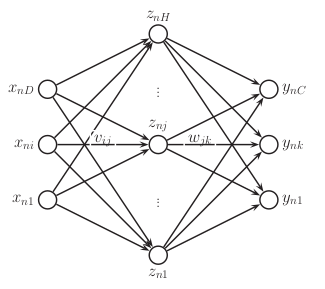
\includegraphics[width=.5\textwidth]{./chapters/3_classical_learning/01_supervised_learning/3_images/1_neural_network_one_hl.png}
    \end{center}
    \caption{caption}
    \label{fig:1_neural_network_one_hl}
\end{figure}
\subparagraph{Convolutional Neural Networks}
It is an MLP in which \tB{the hidden units have local receptive fields}, and in which \tB{the weights
are \emph{tied} or \emph{shared} across the image in order to reduce the number of parameters}. 
Intuitively the \tB{effect of such spatial parameter tying is that any useful features that are 
"discovered" in some portion of the image can be re-used everywhere else without having to be
independently learned}. The resulting network then exhibits \emph{translation invariance} meaning
it can classify patterns no matter where they occur inside the input image.

\paragraph{Strengths}
\paragraph{Weaknesses}
\paragraph{Relationships with other methods}
\paragraph{Examples of application}


%\subsection{Logistic Regression}
%\paragraph{Purpose}
%\paragraph{Assumptions}
%\paragraph{Theory}
%\paragraph{Strengths}
%\paragraph{Weaknesses}
%\paragraph{Relationships with other methods}
%\paragraph{Examples of application}


\section{Model Selection}
\subsection{Bayesian Variable Selection}
\paragraph{Purpose}
Let \tB{$\gamma_{j}: 
\begin{cases}
    \gamma_{j} = 1 \Leftarrow \text{feature } j \text{ is relevant}\\
    \gamma_{j} = 0 \Leftarrow \text{otherwise}\\
\end{cases}$} our goal is to compute the posterior over models:
\begin{center}
    $\prob{\gamma|\mathcal{D}} = \dfrac{e^{-f(\gamma)}}{\su{\gamma'}{}e^{-f(\gamma')}}$
\end{center}
where the cost function is defined by $f(\gamma) \triangleq -\left[\log\left(\prob{
\mathcal{D}|\gamma}\right) + \log\left(\prob{\gamma}\right)\right]$

\paragraph{Assumptions}
\paragraph{Theory}
\subparagraph{Spike and slab model}
remember that posterior is given by $\prob{\bm{\gamma}|\mathcal{D}}\propto \prob{
\mathcal{D}|\bm{\gamma}}\prob{\bm{\gamma}}$.\\
It is common to use the following prior $\prob{\bm{\gamma}} = \prd{j=1}{D}\text{
\emph{Ber}}(\gamma_{j}|\pi_{0}) = \pi_{0}^{\norm{\gamma}_{0}}(1-\pi_{0})^{D-\norm{
\gamma}_{0}}$, where $\pi_{0}$ is the probability that a feature is relevant.\\
The likelihood is defined as follows: $\prob{\mathcal{D}|\bm{X},\bm{\gamma}} = 
\Su{}{}\Su{}{}\prob{\bm{y}|\bm{X},\bm{w},\bm{\gamma}}\prob{\bm{w}|\bm{\gamma},
\sigma^{2}}\prob{\sigma^{2}}d\bm{w}d\sigma^{2}$\\
Consider the prior $\prob{\bm{w}|\bm{\gamma},\sigma^{2}}$ in standardizing the inputs, 
a reasonable prior is $\mathcal{N}(0, \sigma^{2}\sigma_{w}^{2})$, where 
$\sigma_{w}^{2}$ controls how big we expect the coefficients associated with the 
relevant variables to be, which is scaled by the overall noise. We can summarize this 
prior as follows: $\prob{\bm{w}_{j}|\sigma^{2},\gamma_{j}}
\begin{cases}
    \delta_{0}(w_{j}) \Leftarrow \gamma_{j} = 0\\
    \mathcal{N}(w_{j}|0, \sigma^{2}\sigma_{w}^{2}) \Leftarrow \gamma_{j} = 1
\end{cases}$
\uB{the first term is a "spike" at the origin, as $\sigma_{w}^{2}\rightarrow +\infty$ 
the distribution $\prob{w_{j}|\gamma_{j} = 1}$ approaches a uniform distribution which 
can be thought of as a "slab"}.

\subparagraph{Bernoulli-Gaussian model}
we have 
$\begin{cases}
    \prob{y_{i}|\bm{x}_{i},\bm{w}, \bm{\gamma},\sigma^{2}} = \mathcal{N}\left(\su{j}{}
    \gamma_{j}w_{j}x_{ij}, \sigma^{2}\right) \\
    \prob{\gamma_{j}} = \text{\emph{Ber}}(\pi_{0})\\
    \prob{w_{j}} = \mathcal{N}(0, \sigma_{w}^{2})
\end{cases}$
we can think of the \tB{$\gamma_{j}$ as a masking out the weights $w_{j}$}. Unlike the
spike and slab model we do not integrate the irrelevant coefficients, they always 
exists.\\
\uB{One interesting aspect of this model is that it can be used to derive objective 
function that is widely used in the non-Bayesian subset selection literature.}
\subparagraph{Algorithms}
assuming that we want to find the MAP model.
\begin{itemize}
    \item Single best replacement: at each step, we define a \uB{neighborhood of the 
        current model to be all models than can be reached by flipping a single bit
        of $\gamma$}
    \item Orthogonal least squares: we start from an empty set of variables and we 
        add the best feature \tB{$j^{*} = \displaystyle\argmin_{j\notin\bm{\gamma}_{t}}\displaystyle
            \min_{\bm{w}}\norm{\bm{y}-\bm{X}_{\bm{\gamma}_{t}\cup j}\bm{w}}^{2}$} 
    \item Orthogonal matching pursuits: as Orthogonal least squares is somewhat 
        expensive, a simplification is to freeze the current weight and then pick the 
        next feature to add by solving \tB{$j^{*} = \displaystyle\argmin_{j\notin\bm{\gamma}_{t}}
        \displaystyle\min_{\beta} \norm{\bm{y}-\bm{X}\bm{w}_{t} - \beta\bm{x}_{\cdot j}}^{2}$}. And
        $\beta = \dfrac{\bm{x}_{\cdot j}^{T}\bm{r}_{t}}{\norm{\bm{x}_{\cdot j}}^{2}}$, where
        $\bm{r} = \bm{y}-\bm{X}\bm{w}_{t}$
    \item Backward selection: starts with all variables in the model and deletes the
    \item Bayesian matching pursuits: similar to OMP except it uses a Bayesian marginal
        likelihood scoring criterion instead of a least square objective.
\end{itemize}

\paragraph{Strengths}
\paragraph{Weaknesses}
\paragraph{Relationships with other methods}
\paragraph{Examples of application}


\subsection{Least Angle Regression Shrinkage}
\paragraph{Purpose}
Instead of updating only one variable at a time, inducing slow converging, we can use \uB{\emph{
Active set} methods that update many variables at a time}. They add or remove a few variables at
a time so they can take a long time if they started far from the solution.\\
Suppose $\mathcal{A}_{k}$ is the active set of variables at the 
beginning of the $k^{th}$ step and let $\beta_{\mathcal{A}_{k}}$ be the
coefficient vector for these variables at this step, there will be 
$k-1$ nonzero values and the one just entered will be zero.\\
If \uB{$\bm{r}_{k}=\bm{y}-\bm{X}_{\mathcal{A}_{k}}\beta_{\mathcal{A}_{k}}$}
is the current residual, then the direction for this step is:
\begin{center}
    $\delta_{k}=(\bm{X}_{\mathcal{A}_{k}}^{T}\bm{X}_{\mathcal{A}_{k}})^{-1}\bm{X}_{\mathcal{A}_{k}^{T}}^{T}\bm{r}_{k}$
\end{center}
The name ``least angle'' arises from a geometrical interpretation of 
this process; $\bm{u}_{k}$ makes the smallest (and equal) angle with
each of the predictors in $\mathcal{A}_{k}$
\paragraph{Assumptions}
\paragraph{Theory}
Active methods exploit the fact that one can quickly compute $\hat{\bm{w}}(\lambda_{k})$ from 
$\hat{\lambda}(\lambda_{k-1})$ if $\lambda_{k}\approx\lambda_{k-1}$ this is known as \textbf{warm
starting}.

\subparagraph{Least Angle Regression}
\begin{enumerate}
	\item \uB{Standardize the predictors} to have mean zero an unit 
		norm.\\ \uB{Start with the residual $\bm{r}=\bm{y}-
		\overline{\bm{y}}$}, and for all $j\in\inter{1}{p},~\beta_{j}=0$
    \item Find the predictor $x_{j}$ most correlated with $\bm{r}$
    \item For $j\in\inter{1}{p}$
    \begin{itemize}
        \item Move $\beta_{j}$ from 0 to its least-squares coefficient
            $\dfrac{\sP{\bm{x}_{j}}{\bm{r}}}{\sP{\bm{x}_{j}}{\bm{x}_{j}}}$, then recompute 
            $\bm{r}$. Find the predictor $x_{k}$ most correlated with the new $\bm{r}$
        \item Move $\beta_{k}$ from 0 to its least-squares coefficient
            $\dfrac{\sP{\bm{x}_{k}}{\bm{r}}}{\sP{\bm{x}_{k}}{\bm{x}_{k}}}$, then recompute 
            $\bm{r}$. Find the predictor $x_{l}$ most correlated with the new $\bm{r}$\dots
        \item Move $\beta_{j}$ and $\beta_{k}$ in the direction defined
            by their joint least squares coefficient of the current
            residual on $(x_{j},x_{k})$, until some other 
            competitor $x_{l}$ has as much correlation with the
            current residual.
    \end{itemize}
	\item After $\min(N-1, p)$ steps, we arrive at the
		full least-squares solution.
\end{enumerate}

\subparagraph{Least Angle Regression: Lasso Modification}
\begin{itemize}
	\item[4a] If a non-zero coefficient hits zero, drop its variable from the
		active set of varibalbes and recompute the current joint least squares
		direction
\end{itemize}


\paragraph{Strengths}
\begin{itemize}
	\item Numerically efficient when $p\gg n$
	\item As fast as forward selection and has the same order of complexity as OLS
	\item Produces a full piecewise linear solution path
	\item Stable
	\item Esealy modified to produce for other estimators like the Lasso
\end{itemize}

\paragraph{Weaknesses}
\begin{itemize}
    \item Because LARS is based upon iterative refitting of the residuals, it would
		appears to be especially sensitive to the effect noise.
\end{itemize}

\paragraph{Relationships with other methods}
\begin{itemize}
    \item Least Squares
\end{itemize}

\paragraph{Examples of application}


%\subsection{Logistic Regression}
%\paragraph{Purpose}
%\paragraph{Assumptions}
%\paragraph{Theory}
%\paragraph{Strengths}
%\paragraph{Weaknesses}
%\paragraph{Relationships with other methods}
%\paragraph{Examples of application}


\section{Regularization}
\subsection{$l_{1}$ regularization}
\paragraph{Purpose}

\paragraph{Assumptions}
We assume $\prob{\bm{w}|\lambda} = \prd{j=1}{D}\text{\emph{Lap}}(w_{j}|0,
\frac{1}{\lambda}) \propto \prd{j=1}{D}e^{-\lambda|w_{j}|}$
\paragraph{Theory}
For penalized negative log likelihood has the form: $f(\bm{w}) = -\log\left(\prob{
\mathcal{D}|\bm{w}}\right) - \log\left(\prob{\bm{w}|\lambda}\right) = \text{\emph{NLL}}
(\bm{w}) + \lambda\norm{\bm{w}}_{1}$.\\
Geometrically we understand that as we relax the constraint we grow $l_{1}$ ball until
it meets the objective, \tB{the corners of the ball are more likely to intersect the
ellipse than one of the sides} especially in high dimensions because the corners "stick
out". The corners correspond to sparse solutions which lie on the coordinate axes. By
contrast when we grow the $l_{2}$ ball it can intersect the objective at any point, 
there are no "corners" so there is no preference for sparsity. 
\paragraph{Strengths}

\paragraph{Weaknesses}
\begin{itemize}
    \item can give quite different results if the data is slightly perturbed
\end{itemize}
\paragraph{Relationships with other methods}
\paragraph{Examples of application}

\subsection{Regularization path}
\paragraph{Purpose}
As we increase $\lambda$, the solution vector $\hat{\bm{w}}(\lambda)$ will tend to get
sparser, although not necessary monotonically. For each feature $j$ we can plot the 
values $\hat{w}_{j}(\lambda)$ vs $\lambda$ which is known as \emph{regularization path}
\paragraph{Assumptions}
\paragraph{Theory}
\paragraph{Strengths}
\paragraph{Weaknesses}
\paragraph{Relationships with other methods}
\paragraph{Examples of application}

\subsection{Coordinate Descent}
\paragraph{Purpose}
These algorithms exploit the fact that one can quickly compute $\hat{\bm{w}}(
\lambda_{k})$ from $\hat{\bm{w}}(\lambda_{k-1})$ if $\lambda_{k} \approx \lambda_{k-1}$
this is known as \emph{warm starting}.
\paragraph{Assumptions}
\paragraph{Theory}
\subparagraph{Coordinate descent}
$w^{*}_{j} = \argmin_{z}f(\bm{w} + z\bm{e}_{j}) - f(\bm{w})$ with $\bm{e}_{j}$ is the 
\emph{j}'th unit vector. 

\paragraph{Strengths}
\begin{itemize}
    \item if each one-dimensional optimization problem can be solved analitically
\end{itemize}

\paragraph{Weaknesses}
\paragraph{Relationships with other methods}
\paragraph{Examples of application}

%\subsection{Logistic Regression}
%\paragraph{Purpose}
%\paragraph{Assumptions}
%\paragraph{Theory}
%\paragraph{Strengths}
%\paragraph{Weaknesses}
%\paragraph{Relationships with other methods}
%\paragraph{Examples of application}


\section{Ensemble Learning}
The overall purpose is to learn a weighted combination of base models of the form:
\begin{center}
    $f(y|\bm{x},\bm{\pi}) = \su{m\in\mathcal{M}}{}w_{m}f_{m}(y|\bm{x})$
\end{center}
where $w_{m}$ are tunable parameters

\subsection{Boosting}
\paragraph{Purpose}
It aims to \tB{build a model with reduced bias and variance}.\\
It is a greedy algorithm for fitting adaptive basis-function models \tB{$f(\bm{x}) = 
w_{0} + \su{m=1}{M}w_{m}\phi_{m}(\bm{x})$}, where $\phi_{m}$ are generated by an
algorithm called \textbf{weak learner}. \uB{This algorithm works by applying the weak
learner sequentially to weighted versions of the data, where more weight is given to
examples that were misclassified by earlier rounds.}\\
This weak learner can be any classification or regression algorithm, but \tB{it common
to use CART model}.\\
\tB{Boosting is very resistant to overfitting.}\\
The goal of boosting is to solve the following optimization problem:
\begin{center}
    $\displaystyle\min_{f}\su{i=1}{n}L(y_{i},f(\bm{x}_{i}))$
\end{center}

\paragraph{Assumptions}
A \uB{family of \emph{weak learners}} (working slightly better that random guess) 
\uB{can be transformed in a family of \emph{strong learners}}

\paragraph{Theory}
\subparagraph{Forward stagewise additive modeling}
For squared error loss the optimal estimate is given by: $f^{*}(\bm{x}) = \displaystyle
\argmin_{f(\bm{x})}=\mathbb{E}_{y|\bm{x}}\left(\left[y-f(\bm{X}) \right]^{2}\right) = \E{y|\bm{x}}$\\
For binary classification we can use the logloss which is a convex upper bound on 0-1 loss. One can
show that $f^{*}(\bm{x}) = \dfrac{1}{2}\log\left(\dfrac{\prob{\hat{y}=1|\bm{x}}}{\prob{\hat{y}=-1|
\bm{x}}}\right)$

\begin{enumerate}
    \item initialise by defining $f_{0}(\bm{x}) = \displaystyle\argmin_{\gamma}\su{i=1}{n}L\left(
        y_{i},f(\bm{x};\gamma)\right)$, for example if we use squared error we can
        set $f_{0}(\bm{x})=\overline{y}$ and if we use log-loss or exponential loss we can set       
        $f_{0}=\frac{1}{2}\log\left(\frac{\hat{\pi}}{1-\hat{\pi}}\right)$ where $\hat{\pi} = 
        \frac{1}{n}\su{i=1}{n}\mathbbm{1}_{\{y_{i}=1\}}$
    \item at iteration $m$ we compute $(\beta_{m},\gamma_{m}) = \displaystyle\argmin_{\beta,\gamma}
        \su{i=1}{n}L\left(y_{i},f_{m-1}(\bm{x}_{i})+\beta\phi(\bm{x}_{i};\gamma) 
        \right)$ where $\phi$ is generated by the \emph{weak learner} algorithm.
    \item $f_{m}(\bm{x}) = f_{m-1}(\bm{x}) + \nu\beta_{m}\phi(\bm{x}_{i};\gamma_{m})$ where $\nu\in
        [0,1]$ is a step-size parameter.
\end{enumerate}

\begin{center}
    \begin{tabular}{|*{5}{c|}}
    \hline
    \textbf{Name} & \textbf{Loss}& \textbf{Derivate}& \textbf{$f{*}$} & \textbf{Algorithm}\\
    \hline
    \emph{Squared error} & $\frac{1}{2}\left(y_{i}-f(\bm{x}_{i})\right)^{2}$ & 
    $y_{i}-f(\bm{x}_{i})$ & $\E{y|\bm{x}_{i}}$ & \emph{L2Boosting}\\
    \hline
    \emph{Absolute error} & $|y_{i}-f(\bm{x}_{i}|$ & 
    $sgn(y_{i}-f(\bm{x}_{i}))$ & \emph{median}$(y|\bm{x}_{i})$ & \emph{Gradient 
    Boosting}\\
    \hline
    \emph{Exponential loss} & $\exp\left(-y_{i},f(\bm{x}_{i})\right)$ & $-y_{i}\exp(
    -y_{i}f(\bm{x}_{i}))$ & $\frac{1}{2}\log\left(\frac{\pi_{i}}{1 - \pi_{i}}\right)$&
    \emph{AdaBoost}\\
    \hline
    \emph{Logloss} & $\log\left(1+e^{-y_{i}f(\bm{x}_{i})}\right)$ & $-y_{i}-\pi_{i}$ &
    $\frac{1}{2}\log\left(\frac{\pi_{i}}{1 - \pi_{i}}\right)$ & \emph{LogitBoost}\\
    \hline
    \end{tabular}
\end{center}
where $\pi=\sigma\left(2f(\bm{x})\right)$


\paragraph{Strengths}
- robust against overfitting
- reduce bias and variance
\paragraph{Weaknesses}
\paragraph{Relationships with other methods}
\paragraph{Examples of application}


\subsection{Bayes Model Averaging (that is not an Ensemble Method)}
\paragraph{Purpose}
Instead of picking the best model and then using this to make predictions we make
a weighted average of the predictions made by each model:
\paragraph{Assumptions}
\paragraph{Theory}
Let's compute:
\begin{center}
    $\Prob{y|\bm{x},\bm{\mathcal{D}}} = \su{m\in\mathcal{M}}{}
    \Prob{y|\bm{x}, m, \bm{\mathcal{D}}}\Prob{m|\bm{\mathcal{D}}}$
\end{center}
Obviously averaging over all the models is computationally infeasible, then a simple
approximation 
\paragraph{Strengths}
\begin{itemize}
    \item Better results than using any single model
\end{itemize}

\paragraph{Weaknesses}
\paragraph{Relationships with other methods}
\paragraph{Examples of application}


\subsection{Stacking}
\paragraph{Purpose}
Refers to learning a weighted combination of base models of the form:
$f(y|\bm{x},\bm{\pi}) = \su{m\in\mathcal{M}}{}w_{m}f_{m}(y|\bm{x})$ where $w_{m}$ are
the tunable parameters.
\paragraph{Assumptions}
\paragraph{Theory}
To estimate the weights we can use : 
\begin{center}
    $\hat{\bm{w}} = \displaystyle\argmin_{\bm{
w}}\su{i=1}{n}L\left(y_{i},\su{m=1}{M}w_{m}\hat{f}_{m}^{-i}(\bm{x})\right)$
\end{center}
with 
$\hat{f}_{m}^{-i}(\bm{x})$ being the predictor obtained by training on data excluding
$(\bm{x}_{i},y_{i})$. It would allow to avoid overfitting that would produce in using
simply $f_{m}$. This know as \textbf{stacking} or \textbf{stacked generalization}.
\paragraph{Strengths}
\begin{itemize}
    \item Robustness when the "true" model is not in the model class.
\end{itemize}

\paragraph{Weaknesses}
\paragraph{Relationships with other methods}
\paragraph{Examples of application}
\begin{itemize}
    \item analogy with neural networks: $f_{m}$ representing the $m^{th}$ hidden unit 
        and $w_{m}$ are the outputs layer weights
    \item analogy with boosting: where the weights on the base models are determined 
        sequentially
\end{itemize}



\subsection{Boostrap Aggregating (Bagging)}
\paragraph{Purpose}
It is designed to \tB{improve the stability and accuracy} of machine learning 
algorithms.
\paragraph{Assumptions}
\paragraph{Theory}
Let's consider \uB{$M$ different models $\left(f_{m}\right)_{1\leq m\leq M}$} that we 
will train on random different subsets of data (\emph{bootstrap step}).\\
We then compute the ensemble:
\begin{center}
    $f(\bm{x}) = \su{m=1}{M}\dfrac{1}{M}f_{m}(\bm{x})$
\end{center}

\paragraph{Strengths}
\begin{itemize}
    \item Better results than using any single model
\end{itemize}

\paragraph{Weaknesses}
\begin{itemize}
    \item Variance reduction not very efficient because of rerunning same learning
        algorithm on different subsets of the data can result in highly correlated
\end{itemize}


\paragraph{Relationships with other methods}
\begin{itemize}
    \item Random forest: use bagging in randomly cutting the input space vertically 
        (subsets of predictors) and horizontally (subset of observations)
\end{itemize}

\paragraph{Examples of application}



\part{Deep Learning}
% \chapter{Optimization}
\section{Back-propagation}
\subsection{Purpose}
The \tB{back-propagation} algorithm allows the information from the cost to then flow
backwards through the network \tB{in order to compute the gradient}.\\
Actually it refers only to the \tB{method for computing the gradient}, while
\uB{another algorithm such as stochastic gradient descent is used to perform learning}
using this gradient.

\subsection{Modeling}
\paragraph{Chain rule of calculus}
Let $(\bm{x}, \bm{y}) \in \mathbb{R}^{m} \times \mathbb{R}^{n}$ and $z = f(\bm{y})$ 
with $f: \mathbb{R}^{n} \longrightarrow \mathbb{R}$
we have $\nabla_{\bm{x}}z = 
\begin{bmatrix}
    \frac{dz}{dx_{1}}\\
    \vdots \\
    \frac{dz}{dx_{m}}
\end{bmatrix}$,
$\nabla_{\bm{y}}z =
\begin{bmatrix}
    \frac{dz}{dy_{1}}\\
    \vdots \\
    \frac{dz}{dy_{n}}
\end{bmatrix}$ and 
$ \dfrac{\partial\bm{y}}{\partial\bm{x}} = 
\begin{bmatrix}
    \frac{dy_{1}}{x_{1}}  & \cdots & \frac{dy_{1}}{x_{m}}\\
    \vdots                & \ddots & \vdots\\            
    \frac{dy_{n}}{x_{1}}  & \cdots & \frac{dy_{n}}{x_{m}}
\end{bmatrix}$
we have :
\begin{center}
    $\nabla_{\bm{x}}z = \left(\dfrac{\partial\bm{y}}{\partial\bm{x}}\right)^{T}
    \nabla_{\bm{y}}z$
\end{center}

\paragraph{Back-propagation in fully connected MLP}
Consider a network of depth $l$, and the matrices of the model 
$\left(\bm{W}_{j}\right)_{1\leq j\leq l}$ and the bias parameters 
$\left(\bm{b}_{j}\right)_{1\leq j\leq l}$ then $\bm{x}$ the input vector and 
$\bm{y}$ the target vector.

\subparagraph{Forward propagation}
\begin{enumerate}
    \item $\bm{h}_{0} = \bm{x} $
    \item for $k \in \inter{1}{l}$
        \begin{itemize}
            \item $\bm{a}_{k} = \bm{b}_{k} + \bm{W}_{k}\bm{h}_{k-1}$
            \item $\bm{h}_{k} = f(\bm{a}_{k})$
        \end{itemize}
    \item $\hat{\bm{y}} = \bm{h}_{l}$
    \item $J = L(\hat{\bm{y}}, \bm{y}) + \lambda\Omega(\theta)$
        
\end{enumerate}

\subparagraph{Backward}
\begin{enumerate}
    \item $\bm{g} \leftarrow \nabla_{\hat{\bm{y}}}J = \nabla_{\hat{\bm{y}}}L(
        \hat{\bm{y}}, \bm{y})$ 
    \item for $k\in\inter{l-1}{1}$
        \begin{itemize}
            \item $\bm{g} \leftarrow \nabla_{\bm{a}_{k}}\bm{J} = \bm{g}\odot 
                f'(\bm{a}_{k})$
            \item $\nabla_{\bm{b}_{k}}J = \bm{g} + 
                \lambda\nabla_{\bm{b}_{k}}\Omega(\bm{\theta})$
            \item $\nabla_{\bm{W}_{k}}J = \bm{g}\bm{h}^{T}_{k-1}
                + \lambda\nabla_{\bm{W}_{k}}\Omega(\bm{\theta})$
            \item $\bm{g} \leftarrow \nabla_{\bm{h}_{k-1}}J = \bm{W}_{k}^{T}\bm{g}$
        \end{itemize}
        
\end{enumerate}




\chapter{Regularization}
\section{Norm penalities}
We denote the regularized objective function by:
\begin{center}
    $\tilde{J}(\bm{\theta}, \bm{X}, \bm{y}) = J(\bm{\theta}, \bm{X}, \bm{y}) =
    \alpha\Omega(\bm{\theta})$ with 
    $\begin{cases}
        \alpha\in[0,\infty[\text{ hyper-parameters weighting the impact of norm 
        penalty}\\
        \Omega\text{ relative to standard objective function }J
    \end{cases}$
\end{center}

% \subsection{$L^{2}$ parameter regularization}
\paragraph{Purpose}: This penalty is as well knows as \tB{weight decay}, it allows
to drives the weight closer to the origin.

\paragraph{Theory}
$\Omega(\bm{\theta}) = \dfrac{1}{2}\norm{\bm{w}}^{2}_{2}$

\subsection{Data Augmentation}

\subsection{Drop out}
\paragraph{Purpose}
It provides an inexpensive approximation to \tB{training and evaluating a \emph{bagged
ensemble} of exponentially many neural networks}.

\paragraph{Theory}
It \uB{trains the ensemble consisting of \textbf{all sub-networks that can be formed by
removing non-output units}} from an underlying base network.
\begin{figure}[H]
    \begin{center}
        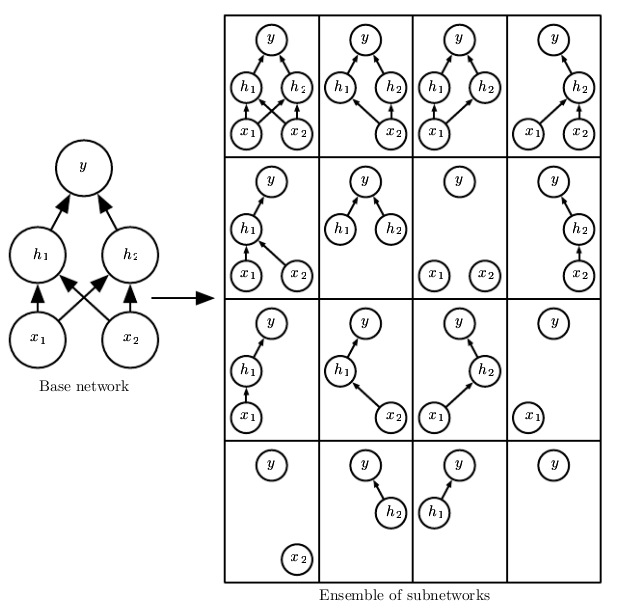
\includegraphics[width=.5\textwidth]{chapters/4_deep_learning/2_regularization/images/01_droupout.png}
    \end{center}
    \caption{Drop out illustration}
    \label{fig:01_droupout.png}
\end{figure}




\chapter{Types of Neural Networks}
\section{Convolutional Neural Networks}
\subsection{Components of CNN}
There are \tB{neural networks using \emph{convolution}} operation instead of general 
matrix multiplication \uB{in at least on of their layers}.
\begin{enumerate}
    \item Apply several convolution in parallel to produce a set of activation 
        functions
    \item The previous activation functions are run through nonlinear activation 
        function (\emph{detector stage})
    \item Modify the output of the layer further with \textbf{pooling functions}
\end{enumerate}

\paragraph{Convolution}
\subparagraph{Convolution operation} \tB{allows to reduce the noise coming from
observation by considering multiple observations and averaging them}. However we want 
to have the \uB{ability to give more weight to some observations}, the more recent ones
for example.
Let's assume we observe \tB{a signal $x(t)$} (\emph{input}) and we have a \tB{weighting
function $w(a) $}(\emph{kernel}) where \uB{$a$ is the age of a measurement} the
resulting signal issued from convolution (\emph{feature map}) is:
\begin{center}
    \tR{$s(t) = (x * w)(t) = \Su{}{}x(a)w(t-a)da$}\\
    or in matrix convention\\
    $\bm{S}(n,p) = \left(\bm{I}*\bm{K}\right)(n, p) = \su{i}{}\su{j}{}\bm{I}(i, j)
    \bm{K}(n-i, p-j) = \su{i}{}\su{j}{}\bm{I}(n-i, p-j) \bm{K}(i, j) =
    \left(\bm{K}*\bm{I}\right)(n, p)$ 
\end{center}
\begin{figure}[H]
    \begin{center}
        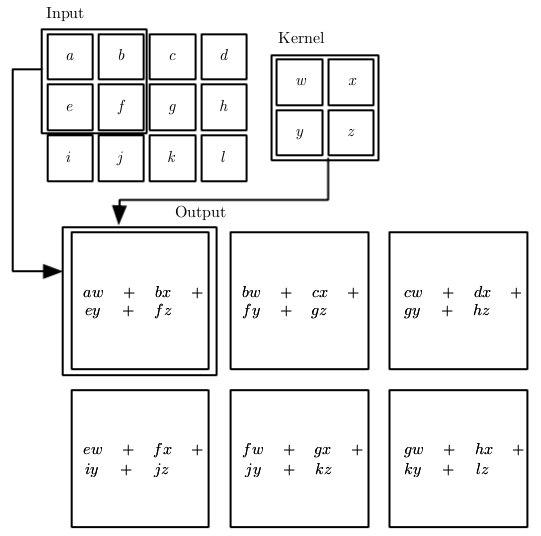
\includegraphics[width=.5\textwidth]{./chapters/4_deep_learning/3_types_of_neural_networks/images/01_convolutional_graph.png}
    \end{center}
    \caption{2-D convolution without kernel-flipping}
    \label{fig:01_convolutional_graph}
\end{figure}

\subparagraph{Motivation}
\begin{itemize}
    \item \textbf{sparse interactions} (due to reduced size of kernel compare with the 
        input one)
    \item \textbf{parameter sharing} (rather than learning a separate set of 
        parameters, for every location we learn only one set, that are the kernel's 
        ones)
    \item \textbf{equi-variant representations}: \tG{$f(x)$ is equi-variant to a
            function $g$ if $f\left(g(x)\right) = g\left(f(x)\right)$}. For example 
            \uB{if $g$ is any function that translates the input then the convolution 
            is equi-variant to $g$}
        \begin{itemize}
            \item for time series, \tB{convolution produces a sort of timeline showing
                when different features appear in the input}.\\
                By moving an event later in time in the input will induce that the same
                representation of the event will appear in the output
            \item for images, \tB{convolution creates a 2-D map of where certain 
                features appear in the input}.\\
                By moving the object in the input, its representation will move the 
                same amount in the output
        \end{itemize}
    \item \textbf{ability to work with inputs of variable size}
\end{itemize}


\paragraph{Pooling}
\subparagraph{Purpose} of pooling is to \tB{make representation become approximately
\emph{invariant} to small translations of the input}. Such a priority can be very
useful when we are searching for the presence of some feature rather than their 
location.\\
It can be viewed as \uB{adding an infinitely strong prior to the weight resulting in 
layer invariance} to small translations

\subparagraph{Examples of pooling}
\begin{figure}[H]
    \begin{center}
        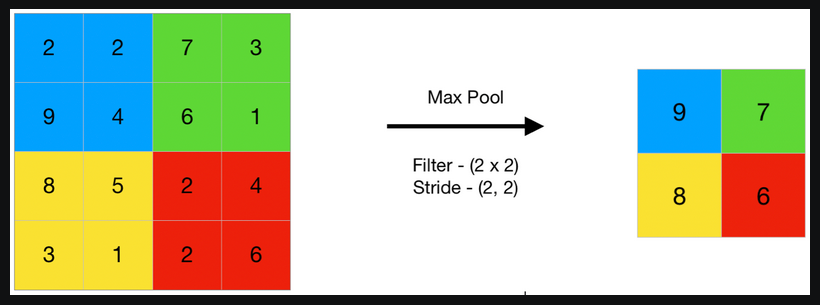
\includegraphics[width=.5\textwidth]{./chapters/4_deep_learning/3_types_of_neural_networks/images/02_pooling_max.png}
    \end{center}
    \caption{Max pooling}
    \label{fig:02_pooling_max}
\end{figure}


\begin{figure}[H]
    \begin{center}
        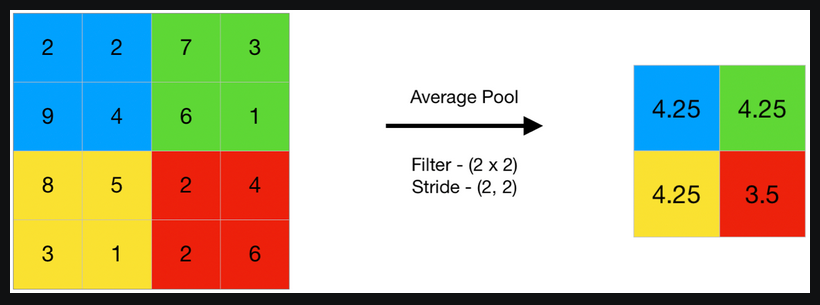
\includegraphics[width=.5\textwidth]{./chapters/4_deep_learning/3_types_of_neural_networks/images/02_pooling_average.png}
    \end{center}
    \caption{Max pooling}
    \label{fig:02_pooling_average}
\end{figure}


\section{Recurrent and Recursive Neural Networks}
\subsection{Recurrent Neural Networks}
\paragraph{Architecture}, let's consider a \emph{computational graph} to compute the
training loss of a recurrent neural network that maps an input sequence of $\bm{L}$ to 
a corresponding sequence of output $\bm{o}$ values. A loss $\bm{L}$ measures how far each
$\bm{o}$ is from the corresponding  training target $\bm{y}$
\begin{figure}[H]
    \begin{center}
        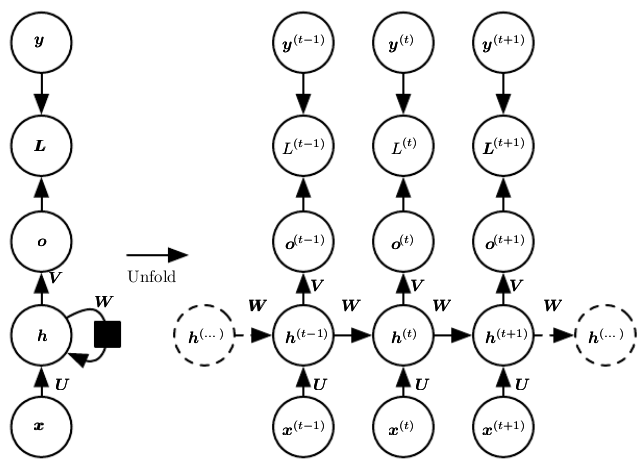
\includegraphics[width=.5\textwidth]{chapters/4_deep_learning/3_types_of_neural_networks/images/03_rnn.png}
    \end{center}
    \caption{Recurrent Neural Networks}
    \label{fig:03_rnn}
\end{figure}


\subsection{Encoder-Decoder Sequence-to-Sequence Architectures}

It is composed of an \uB{encoder RNN that reads} the input sequence and a \uB{decoder
RNN that generates} the output sequence.
\begin{figure}[H]
    \begin{center}
        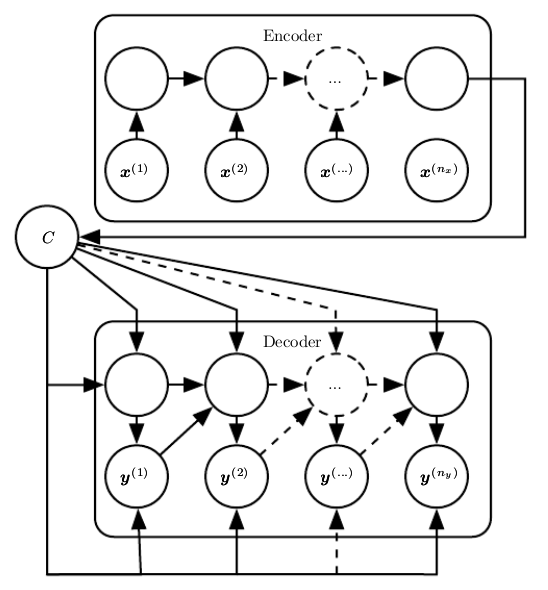
\includegraphics[width=.5\textwidth]{chapters/4_deep_learning/3_types_of_neural_networks/images/03_encoder_decoder_architecture.png}
    \end{center}
    \caption{Encoder-Decoder (or Sequence-to-Sequence RNN) architecture}
    \label{fig:03_encoder_decoder_architecture}
\end{figure}

The \tR{final hidden state of the encoder RNN is used to compute a generally fixed-size
context variable $C$ representing a semantic summary of the input sequence}, then is
given as input to the decoder RNN.

\subsection{The Challenge of Long-Term Dependencies}
\paragraph{The basic problem} is that \uB{gradients propagated over many stages tend to
either vanish or explode}.\\
Consider a very simple recurrent neural network network lacking a nonlinear function:
$\bm{h}_{t} = \bm{W}^{T}\bm{h}_{t-1}$, if we admits an eigen-decomposition of the form
$\bm{W} = \bm{Q}\bm{\Lambda}\bm{Q}^{T}$ with orthogonal $\bm{Q}$ the recurrence may be
simplified further to $\bm{h}_{t} = \bm{Q}^{T}\bm{\Lambda}^{t}\bm{Q}\bm{h}_{0}$.
\uB{The eigenvalues are raised to the power of $t$ causing the eigenvalues with
magnitude lesser than one to decay to zero and eigenvalues with magnitude greater than 
one to explode}.

\subsection{Leaky Units}
\paragraph{Purpose} dealing with long-term dependencies by designing a model operating
at multiple time scales, allowing to \uB{let some parts of the model operating at 
fine-grained time scales to handle small details while other parts operate at coarse
time scales and transfer information from the distant past to the present more 
efficiently}.

\subparagraph{Adding Skip Connections through Time} consists in \uB{adding direct 
connections from variables in the distant past to variables in the present}.\\
By introducing recurrent connections with a time-delay of $d$ to mitigate,
\tB{Gradients now diminish exponentially as a function of $\frac{\tau}{d}$ rather than
$\tau$}

\paragraph{Leaky Units}
Another way to obtain paths on which the product of derivatives is close to one is to
\tB{have units with linear self-connections} and a weight near one on these
connections.
When we accumulate a running average $\mu_{t}$ of some value $v_{t}$ by applying
$\mu_{t} \leftarrow \alpha\mu_{t-1} + (1-\alpha)v_{t}$ the $\alpha$ parameter is an
example of linear self connection from $\mu_{t-1}$ to $\mu_{t}$.\\
\tB{When $\alpha$ is near one, the running average remembers information about the past
for a long time, and when $\alpha$ is near zero, information about the past is 
rapidly discarded}.



\subsection{The Long Short-Term Memory (LSTM) and Gated Recurrent Unit (GRU)}
\paragraph{Purpose}
going further with the idea of self-loops, by making the weight of the self-loop
conditioned on the context rather than fixed.\\
\tB{Self-loops produce paths where the grdient can flow for long duration}.

\begin{figure}[H]
    \begin{center}
        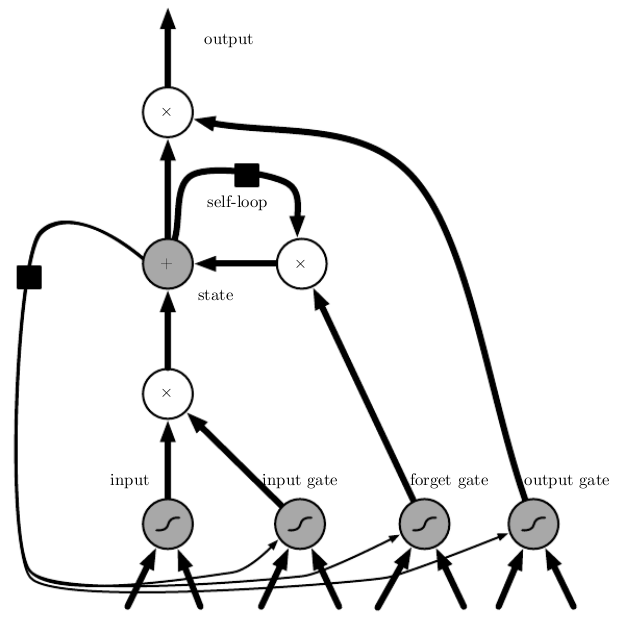
\includegraphics[width=.5\textwidth]{chapters/4_deep_learning/3_types_of_neural_networks/images/04_lstm_rnn_cell.png}
    \end{center}
    \caption{Block diagram of the LSTM recurrent neural network \emph{cell}}
    \label{fig:label}
\end{figure}

Cells are connected recurrently to each other replacing the usual hidden units of
ordinary recurrent networks.

\paragraph{Theory}
The \textbf{forget gate} unit $f_{i}^{(t)}$ for time step $t$ and cell $i$ that sets
the weight to a value between 0 and 1
\begin{center}
    \frB{$f_{i}^{t} = \sigma\left(b_{i}^{f} + \su{j}{}U_{i,j}^{f}x_{j}^{(t)} +
    \su{j}{}W_{i,j}^{f}h_{j}^{(t-1)}\right)$}
\end{center}
with $\bm{x}^{(t)}$ the current input vector, $\bm{h}^{t}$ the current hidden layer vector
containing the outputs of all the LSTM cells, and $\bm{b}^{f},~\bm{U}^{f},~\bm{W}^{f}$ are
respectively biases, input weights and recurrent weights for the forget gates.



%   - Gradient based approach
%   - Direct feedback alignment
%   - Forward forward algorithm

% \chapter{Regularization}
% \chapter{General notions in neural Networks}
%   - Components
%       - Activation functions
%       - Hidden layers
% \chapter{Types of neural networks}
%   - FFNN
%      - purpose
%      - theory
%      - advantages
%      - disadvantages
%      - link to other algorithms
%      - application 
%   - CNN
%   - RNN
%   - AE
%   - DBN
% \chapter{Complex Architecture}
%    - Transformers
%      - GPT
%      - BERT

% \chapters{Components}
% Layers
    % Activation functions

\part{Overall Issues}
\section{High Dimensions}
\subsection{Dimension Increase}
\subsection{Curse of dimensionality}
\paragraph{Purpose}
When the dimensionality increases, the \tB{volume of the space increases so fast that the available 
data become sparse}.
\paragraph{Main issues}
\subparagraph{Combinatorics}
Let's consider $(d,k)\in\mathbb{N}^{*}$ and $(x_{i})_{1\leq i\leq d} \in\inter{1}{K}^{d}$, the
range of possible values for the families $(x_{i})_{1\leq i\leq d}$ is $K^{d}$  which increases 
obviously exponentially.






\printbibliography

\end{document}
